% Template KLTN cho SV trường ĐHKHTN
% Liên hệ: nqminh@fit.hcmus.edu.vn
% Last update: 08/06/2016

% Chú ý: đọc các phần chú ý đóng khung của file này và chỉnh lại cho phù hợp.
% Trước khi build, xóa hết các file được tạo ra trong quá trình build trước đó, và build theo thứ tự: BIB > PDF > PDF.
% Nếu cập nhật tài liệu tham khảo, cũng cần build lại theo cách trên.

\documentclass[oneside,a4paper,14pt]{extreport}

% Font tiếng Việt
\usepackage[T5]{fontenc}
\usepackage[utf8]{inputenc}
\DeclareTextSymbolDefault{\DH}{T1}


% Tài liệu tham khảo
\usepackage[
	sorting=nty,
	backend=bibtex,
	defernumbers=true]{biblatex}
\usepackage[unicode]{hyperref} % Bookmark tiếng Việt
\addbibresource{References/references.bib}

\makeatletter
\def\blx@maxline{77}
\makeatother

% Chèn hình, các hình trong luận văn được để trong thư mục Images/
\usepackage{graphicx}
\graphicspath{ {Images/} }

% Chèn và định dạng mã nguồn
\usepackage{listings}
\usepackage{color}
\definecolor{codegreen}{rgb}{0,0.6,0}
\definecolor{codegray}{rgb}{0.5,0.5,0.5}
\definecolor{codepurple}{rgb}{0.58,0,0.82}
\definecolor{backcolour}{rgb}{0.95,0.95,0.92}
\lstdefinestyle{mystyle}{
    backgroundcolor=\color{backcolour},   
    commentstyle=\color{codegreen},
    keywordstyle=\color{magenta},
    numberstyle=\tiny\color{codegray},
    stringstyle=\color{codepurple},
    basicstyle=\footnotesize,
    breakatwhitespace=false,         
    breaklines=true,                 
    captionpos=b,                    
    keepspaces=true,                 
    numbers=left,                    
    numbersep=5pt,                  
    showspaces=false,                
    showstringspaces=false,
    showtabs=false,                  
    tabsize=2
}
\lstset{style=mystyle}

% Chèn và định dạng mã giả
\usepackage{amsmath}
\usepackage{algorithm}
\usepackage[noend]{algpseudocode}
\makeatletter
\def\BState{\State\hskip-\ALG@thistlm}
\makeatother

% Do-while speudocode
\usepackage{algorithmicx}
\usepackage{algpseudocode}


\algdef{SE}[DOWHILE]{Do}{doWhile}{\algorithmicdo}[1]{\algorithmicwhile\ #1}%

\usepackage{amsfonts}
\usepackage{amssymb}

% Bảng biể
\usepackage{booktabs}
\usepackage{multirow}
\usepackage{array}
\newcolumntype{L}[1]{>{\raggedright\let\newline\\\arraybackslash\hspace{0pt}}m{#1}}
\newcolumntype{C}[1]{>{\centering\let\newline\\\arraybackslash\hspace{0pt}}m{#1}}
\newcolumntype{R}[1]{>{\raggedleft\let\newline\\\arraybackslash\hspace{0pt}}m{#1}}

% Đổi tên mặc định
\renewcommand{\chaptername}{Chương}
\renewcommand{\figurename}{Hình}
\renewcommand{\tablename}{Bảng}
\renewcommand{\contentsname}{Mục lục}
\renewcommand{\listfigurename}{Danh sách hình}
\renewcommand{\listtablename}{Danh sách bảng}
\renewcommand{\appendixname}{Phụ lục}


% Dãn dòng 1.5
\usepackage{setspace}
\onehalfspacing

% Thụt vào đầu dòng
\usepackage{indentfirst}

% Canh lề
\usepackage[
  top=30mm,
  bottom=25mm,
  left=30mm,
  right=20mm,
  includefoot]{geometry}
  
% Trang bìa
\usepackage{tikz}
\usetikzlibrary{calc} 
\newcommand\HRule{\rule{\textwidth}{1pt}}

% ========================================================================================= %
% CHÚ Ý: Thông tin chung về KLTN - sinh viên điền vào đây để tự động update các trang khác  %
% ========================================================================================= %
\newcommand{\tenSV}{Ngô~Phù~Hữu~Đại~Sơn} % Dấu ~ là khoảng trắng không được tách (các chữ nối với nhau bằng dấu ~ sẽ nằm cùng 1 dòng
\newcommand{\mssv}{18120078}
\newcommand{\tenKL}{Sử dụng GNN để tăng độ hiệu quả của bài toán Machine Translation} % Chú ý dấu ~ trong tên khóa luận
\newcommand{\tenGVHD}{Nguyễn Ngọc Thảo}
\newcommand{\tenBM}{Khoa học máy tính}

\begin{document}

\begin{titlepage}

\begin{center}
%ĐẠI HỌC QUỐC GIA THÀNH PHỐ HỒ CHÍ MINH\\
TRƯỜNG ĐẠI HỌC KHOA HỌC TỰ NHIÊN\\
\textbf{KHOA CÔNG NGHỆ THÔNG TIN}\\[2cm]


{ \Large \bfseries \tenSV\\[2cm] } 

%Tên đề tài Khóa luận tốt nghiệp/Đồ án tốt nghiệp

{ \Large \bfseries \tenKL \\[3cm]} 


%Chọn trong các dòng sau
% \large LUẬN VĂN THẠC SĨ KHOA HỌC MÁY TÍNH\\
\large KHÓA LUẬN TỐT NGHIỆP CỬ NHÂN\\
%\large THỰC TẬP TỐT NGHIỆP CỬ NHÂN\\
%Đưa vào dòng này nếu thuộc chương trình Chất lượng cao, hoặc lớp Cử nhân tài năng
\large CHƯƠNG TRÌNH CHÍNH QUY\\
%\large CHƯƠNG TRÌNH CHẤT LƯỢNG CAO\\
%\large CHƯƠNG TRÌNH CỬ NHÂN TÀI NĂNG\\[2cm]


\begin{tikzpicture}[remember picture, overlay]
  \draw[line width = 2pt] ($(current page.north west) + (2cm,-2cm)$) rectangle ($(current page.south east) + (-1.5cm,2cm)$);
\end{tikzpicture}

\vfill
Tp. Hồ Chí Minh, tháng 07/2022

\end{center}

\pagebreak



\begin{center}

TRƯỜNG ĐẠI HỌC KHOA HỌC TỰ NHIÊN\\
\textbf{KHOA CÔNG NGHỆ THÔNG TIN}\\[2cm]


{\large \bfseries Ngô Phù Hữu Đại Sơn - \mssv\\} 


%Tên đề tài Khóa luận tốt nghiệp/Đồ án tốt nghiệp

{ \Large \bfseries \tenKL\\[2cm]}  


%Chọn trong các dòng sau
% \large LUẬN VĂN THẠC SĨ KHOA HỌC MÁY TÍNH\\
\large KHÓA LUẬN TỐT NGHIỆP CỬ NHÂN\\
%Đưa vào dòng này nếu thuộc chương trình Chất lượng cao, hoặc lớp Cử nhân tài năng
\large CHƯƠNG TRÌNH CHÍNH QUY\\[2cm]
%\large CHƯƠNG TRÌNH CHẤT LƯỢNG CAO\\[2cm]
%\large CHƯƠNG TRÌNH CỬ NHÂN TÀI NĂNG\\[2cm]

\textbf{NGƯỜI HƯỚNG DẪN}\\
TS. \tenGVHD\\
ThS. Tạ Việt Phương \\


\begin{tikzpicture}[remember picture, overlay]
  \draw[line width = 2pt] ($(current page.north west) + (2cm,-2cm)$) rectangle ($(current page.south east) + (-1.5cm,2cm)$);
\end{tikzpicture}

\vfill
Tp. Hồ Chí Minh, tháng 07/2022

\end{center}

\end{titlepage}
% Sasu trang Title, các bạn chèn nhận xét gủa GVHD và GVPB. Nhận xét sẽ được giáo vụ phát sau buổi bảo vệ để các bạn đóng quyển.

\pagenumbering{roman} % Đánh số i, ii, iii, ...

%\addcontentsline{toc}{chapter}{Lời cam đoan}
%\chapter*{Lời cam đoan}
\label{reassurances}

Sinh viên xin cam đoan đây là công trình nghiên cứu của riêng sinh viên. Các số liệu và kết quả nghiên cứu trong luận văn này là trung thực và không trùng lặp với các đề tài khác.

\addcontentsline{toc}{chapter}{Lời cảm ơn}
\chapter*{Lời cảm ơn}
\label{thanks}

Trải qua thời gian dài học tập trong trường, đã đến lúc những kiến thức của em được vận dụng vào thực tiễn công việc. Em lựa chọn làm khóa luận tốt nghiệp để tổng hợp lại kiến thức của mình. Đề tài của em là: “\textit{\tenKL}”. Trong suốt quá trình làm khóa luận, em đã nhận được sự hướng dẫn, giúp đỡ quý báu của các thầy cô, các anh chị và các bạn. Em xin được bày tỏ lời cảm ơn chân thành tới:

TS \tenGVHD\ đã hướng dẫn và truyền đạt những kinh nghiệm quý báu cho em trong suốt thời gian làm khóa luận tốt nghiệp của mình.

Em cũng cảm ơn gia đình và bạn bè đã giúp đỡ em hoàn thành tốt khóa luận.

Khóa luận của em còn những hạn chế về năng lực và những thiếu sót trong quá trình nghiên cứu. Em xin lắng nghe và tiếp thu những ý kiến của giáo viên phản biện để hoàn thiện, bổ sung kiến thức.

Em xin chân thành cảm ơn!

\addcontentsline{toc}{chapter}{Đề cương chi tiết}
\include{Appendix/decuong}

% Mục lục, danh sách hình, danh sách bảng
\addcontentsline{toc}{chapter}{Mục lục}
\tableofcontents
\listoffigures
\listoftables

\addcontentsline{toc}{chapter}{Tóm tắt}
\chapter*{Tóm tắt}
\label{abstract}

Trong quá trình phát triển của công nghệ ngày nay, nhu cầu được kết nối với mọi người, mọi loại thông tin trên khắp thế giới là một nhu cần thiết cho tất cả mọi người. Một trong những rào cản để kết nối giữa các thực thể ở cách xa nhau về vùng địa lý chính là ngôn ngữ. Do đó, bài toán về dịch máy ngày càng trở nên quan trọng và cần được xử lý một cách hiệu quả.

Mô hình \textit{Transformer} là một trong các mô hình được đánh giá là cho ra kết quả tốt cho bài toán dịch máy vào những năm gần đây. Mô hình hoàn toàn dựa trên cơ chế attention thay vì sử dụng các kiến trúc hồi quy hay tích chập vốn đã cho ra các kết quả tốt trước đây.

Trong những năm gần đây, các thuật toán học máy đang được phát triển trên các bộ dữ liệu đồ thị. Trong đó, có kiến trúc mạng \textit{Graph Convolutional Network (GCN)} được đánh giá là một trong những kiến trúc quan trọng trong việc giải các bài toán học máy trên đồ thị. 

Hướng tiếp cận của khóa luận này là áp dụng được mô hình \textit{Graph Convolutional Network} vào mô hình dịch máy (cụ thể là \textit{Transformer}) để tăng tính hiệu quả và tăng tốc độ hội tụ của mô hình. 

\clearpage

\pagenumbering{arabic} % Đánh số 1, 2, 3, ...

% Các chương nội dung
\chapter{Giới thiệu}
\label{Chapter1}

%Tóm tắt luận văn được trình bày nhiều nhất trong 24 trang in trên hai mặt giấy, cỡ chữ Times New Roman 11 của hệ soạn thảo Winword hoặc phần mềm soạn thảo Latex đối với các chuyên ngành thuộc ngành Toán.

%Mật độ chữ bình thường, không được nén hoặc kéo dãn khoảng cách giữa các chữ.
%Chế độ dãn dòng là Exactly 17pt.
%Lề trên, lề dưới, lề trái, lề phải đều là 1.5 cm.
%Các bảng biểu trình bày theo chiều ngang khổ giấy thì đầu bảng là lề trái của trang.
%Tóm tắt luận án phải phản ảnh trung thực kết cấu, bố cục và nội dung của luận án, phải ghi đầy đủ toàn văn kết luận của luận án.
%Mẫu trình bày trang bìa của tóm tắt luận văn (phụ lục 1).

\section{Đặt vấn đề}
Ngôn ngữ là một loại phương tiện giúp con người có thể giao tiếp và truyền đạt suy nghĩ, ý kiến của mình cho những người xung quanh. Theo trang \textit{Ethnologue.com}\cite{Ethnologue}, tính đến năm 2022, trên thế giới có 7151 ngôn ngữ. Vì vậy, một người không thể nào học và hiểu hết mọi ngôn ngữ trên thế giới. Từ đó, có thế độ cần thiết của việc dịch từ một ngôn ngữ sang một ngôn ngữ khác. Ngành khoa học máy tính, cụ thể hơn là xử lý ngôn ngữ tự nhiên, chúng ta cũng quan tâm đến bài toán trên.

\begin{figure}[H]
    \begin{center}
        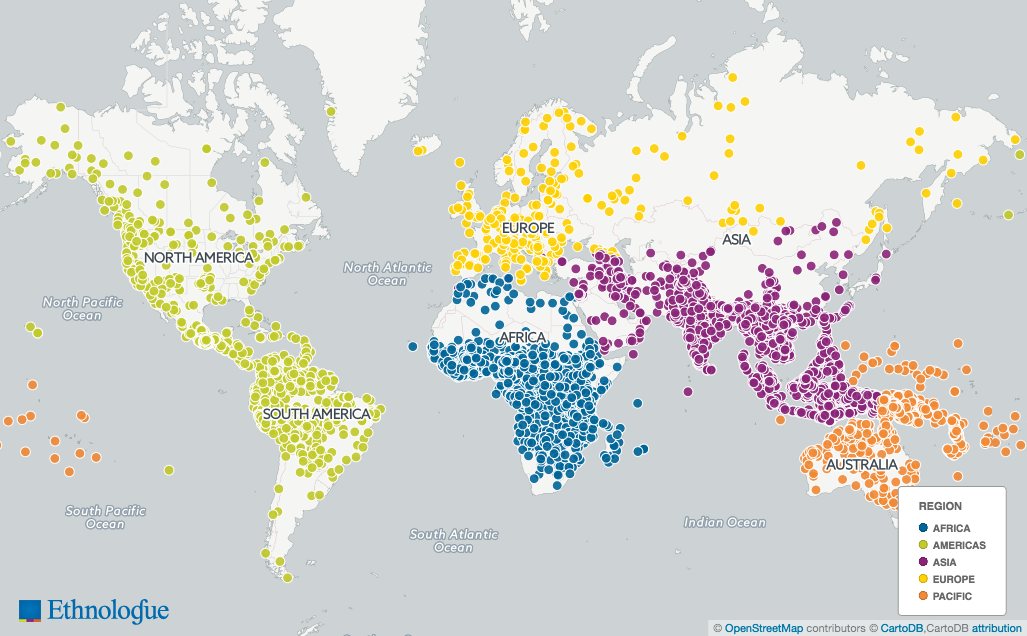
\includegraphics[scale=0.4]{images/number_of_langs}
        \caption{Phân bố các ngôn ngữ trên thế giới\cite{Ethnologue}}
        \label{fig:languages_distibuttion}
    \end{center}
\end{figure}

\section{Bài toán dịch máy (Machine Translation)}

Bài toán dịch máy là một lĩnh vực trong ngành khoa học máy tính. Đầu vào được nhập vào máy tính là một đoạn văn bản từ một ngôn ngữ (ngôn ngữ nguồn). Và qua quá trình xử lý, đưa ra được đoạn văn bản tương ứng ở một ngôn ngữ khác (ngôn ngữ đích). Khác với các mô hình xử lý ngôn ngữ khác, khi chúng chỉ cần một kho ngữ liệu của một ngôn ngữ. Các mô hình dịch máy cần ít nhất hai kho ngữ liệu của ngôn ngữ nguồn và ngôn ngữ đích. kho ngữ liệu bao gồm tập các đoạn văn bản. Với mỗi đoạn văn bản từ ngôn ngữ nguồn sẽ được ánh xạ đến một đoạn văn bản có ý nghĩa tương ứng ở ngôn ngữ đích. Các kho ngữ liệu này có thể tổng hợp từ các nguồn khác nhau: từ các bản dịch (subtitle) của các bộ phim, bản dịch sách và cả các bộ dữ liệu được thiết kế riêng cho bài toàn dịch máy (các bản dịch từ các chuyên gia).

Để có thể hiểu hơn sâu hơn bài toán và tìm ra hướng giải quyết, ta cần phải hiểu được cách tự nhiên mà con người dịch một đoạn văn bản từ ngôn ngữ nguồn sang ngôn ngữ đích như thế nào. Theo như \cite{2014arXiv1409.0473B}, quá trình này có thể chia làm hai bước:
\begin{itemize}
	\item Trích xuất ngữ cảnh, văn cảnh (\textit{context}) của ngôn ngữ nguồn thành thông tin.
	\item Chuyển hóa thông tin thu thập được thành ngôn ngữ đích.
\end{itemize}

\section{Các cách tiếp cận trước}

Với tính chất trên của bài toán, ta có thể thấy bài toán này là một bài toán \textit{sequence-to-sequence(Seq2Seq)} và có thể giải quyết bằng kiến trúc \textit{encoder-decoder}. Các mô hình sử dụng các mạng nơ ron hồi quy (Recursive Neural Network) sử dụng cơ chế Long-Short-Term-Memory.

\begin{figure}[H]
    \begin{center}
        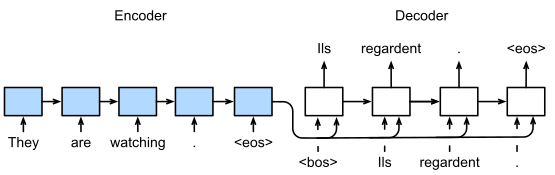
\includegraphics[scale=0.8]{images/seq2seq}
        \caption{Tổng quan kiến trúc mô hình Seq2Seq \cite{seq2seq}}
        \label{fig:seq2seq}
    \end{center}
\end{figure}


Các mô hình hồi quy (\textit{Recurrent model}) cho các kết quả tốt trong bài toán dịch máy. Tuy nhiên, các mô hình này lại sử dụng cơ chế hồi quy. Ở mỗi bước tính toán, mô hình sử dụng thông tin ẩn (\textit{hidden state}) được tổng hợp từ đầu văn bản đến hiện tại $h_t$ để làm đầu vào tính toán. Quá trình này lặp lại cho mỗi bước. Từ đó, ta có thể thấy mô hình tính toán bước tiếp theo phải phụ thuộc vào bước trước đó, dẫn đến không thể song song quá trình tính toán này được. Điều này khiến cho việc tối ưu thời gian huấn luyện lẫn hiệu quả tính toán của mô hình trước nên khó khăn.

\begin{figure}[H]
    \begin{center}
        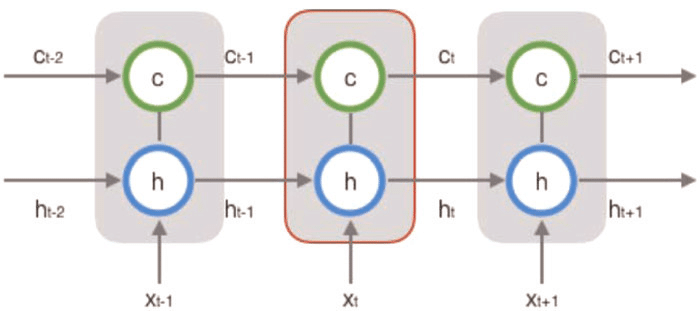
\includegraphics[scale=0.6]{images/hidden-state}
        \caption{Kiến trúc \textit{mạng hồi quy} với các thông tin ẩn}
        \label{fig:hidden state}
    \end{center}
\end{figure}

Một nhược điểm khác của các mô hình hồi quy đó là dễ xảy ra hiện tượng \textit{Gradient biến mất} (\textit{Gradient Vanishing}) và đôi khi là \textit{Gradient bùng nổ}(\textit{Gradient Exploding}). Nguyên nhân cốt lõi của vấn đề này là do công thức của hàm phi tuyến chưa hợp lý làm cho quá trình lan truyền ngược (\textit{back propagation}), các giá trị \textit{gradient} của mỗi lớp quá lớn hoặc quá nhỏ. Do đó làm cho \textit{gradient} lan truyền về sau trở nên càng lớn hoặc càng nhỏ theo cấp số mũ. Vấn đề \textit{Gradient biến mất} sẽ làm cho mô hình hồi tụ chậm đi khi mô hình học sâu được tăng thêm số lớp. Để giải quyết vấn đề này, kiến trúc \textit{LSTM (long short term memory)} được giới thiệu. Với \textit{LSTM}, hiện tượng \textit{Gradient biến mất} được cải thiện. Do đó khi mô hình đang xử lý ở bước thứ $i$, các thông tin từ các bước trước đó không bị mất đi. Nhờ vậy mà quá trình học ở bước hiện tại trở nên hiệu quả hơn.

\begin{figure}[H]
    \begin{center}
        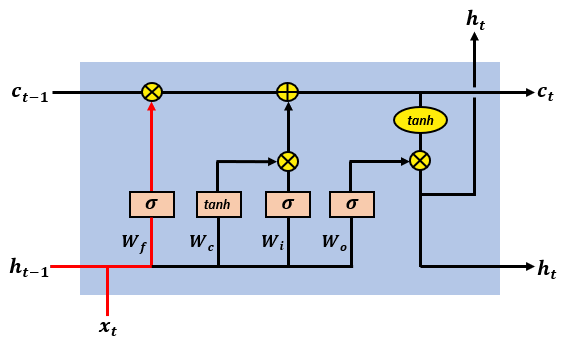
\includegraphics[scale=0.6]{images/lstm}
        \caption{Kiến trúc \textit{LSTM} \cite{lstm}}
        \label{fig:lstm}
    \end{center}
\end{figure}

\section{transformer}

\textit{Transformer} \cite{transformer} - một phương pháp dựa hoàn toàn trên cơ chế attention, bỏ qua các cấu trúc của mạng nơ ron hồi quy và mạng nơ ron tích chập phức tạp, giúp đơn giản hóa mô hình những vẫn thể hiện được độ hiệu quả của mô hình. Theo \textbf{Paper attention is all your need} \cite{transformer}, mô hình cho kết quả 41.8 BLEU khi huấn luyện trên tập WMT 2014, cao hơn tất cả các mô hình dịch máy trước đó. 

\begin{figure}[H]
    \begin{center}
        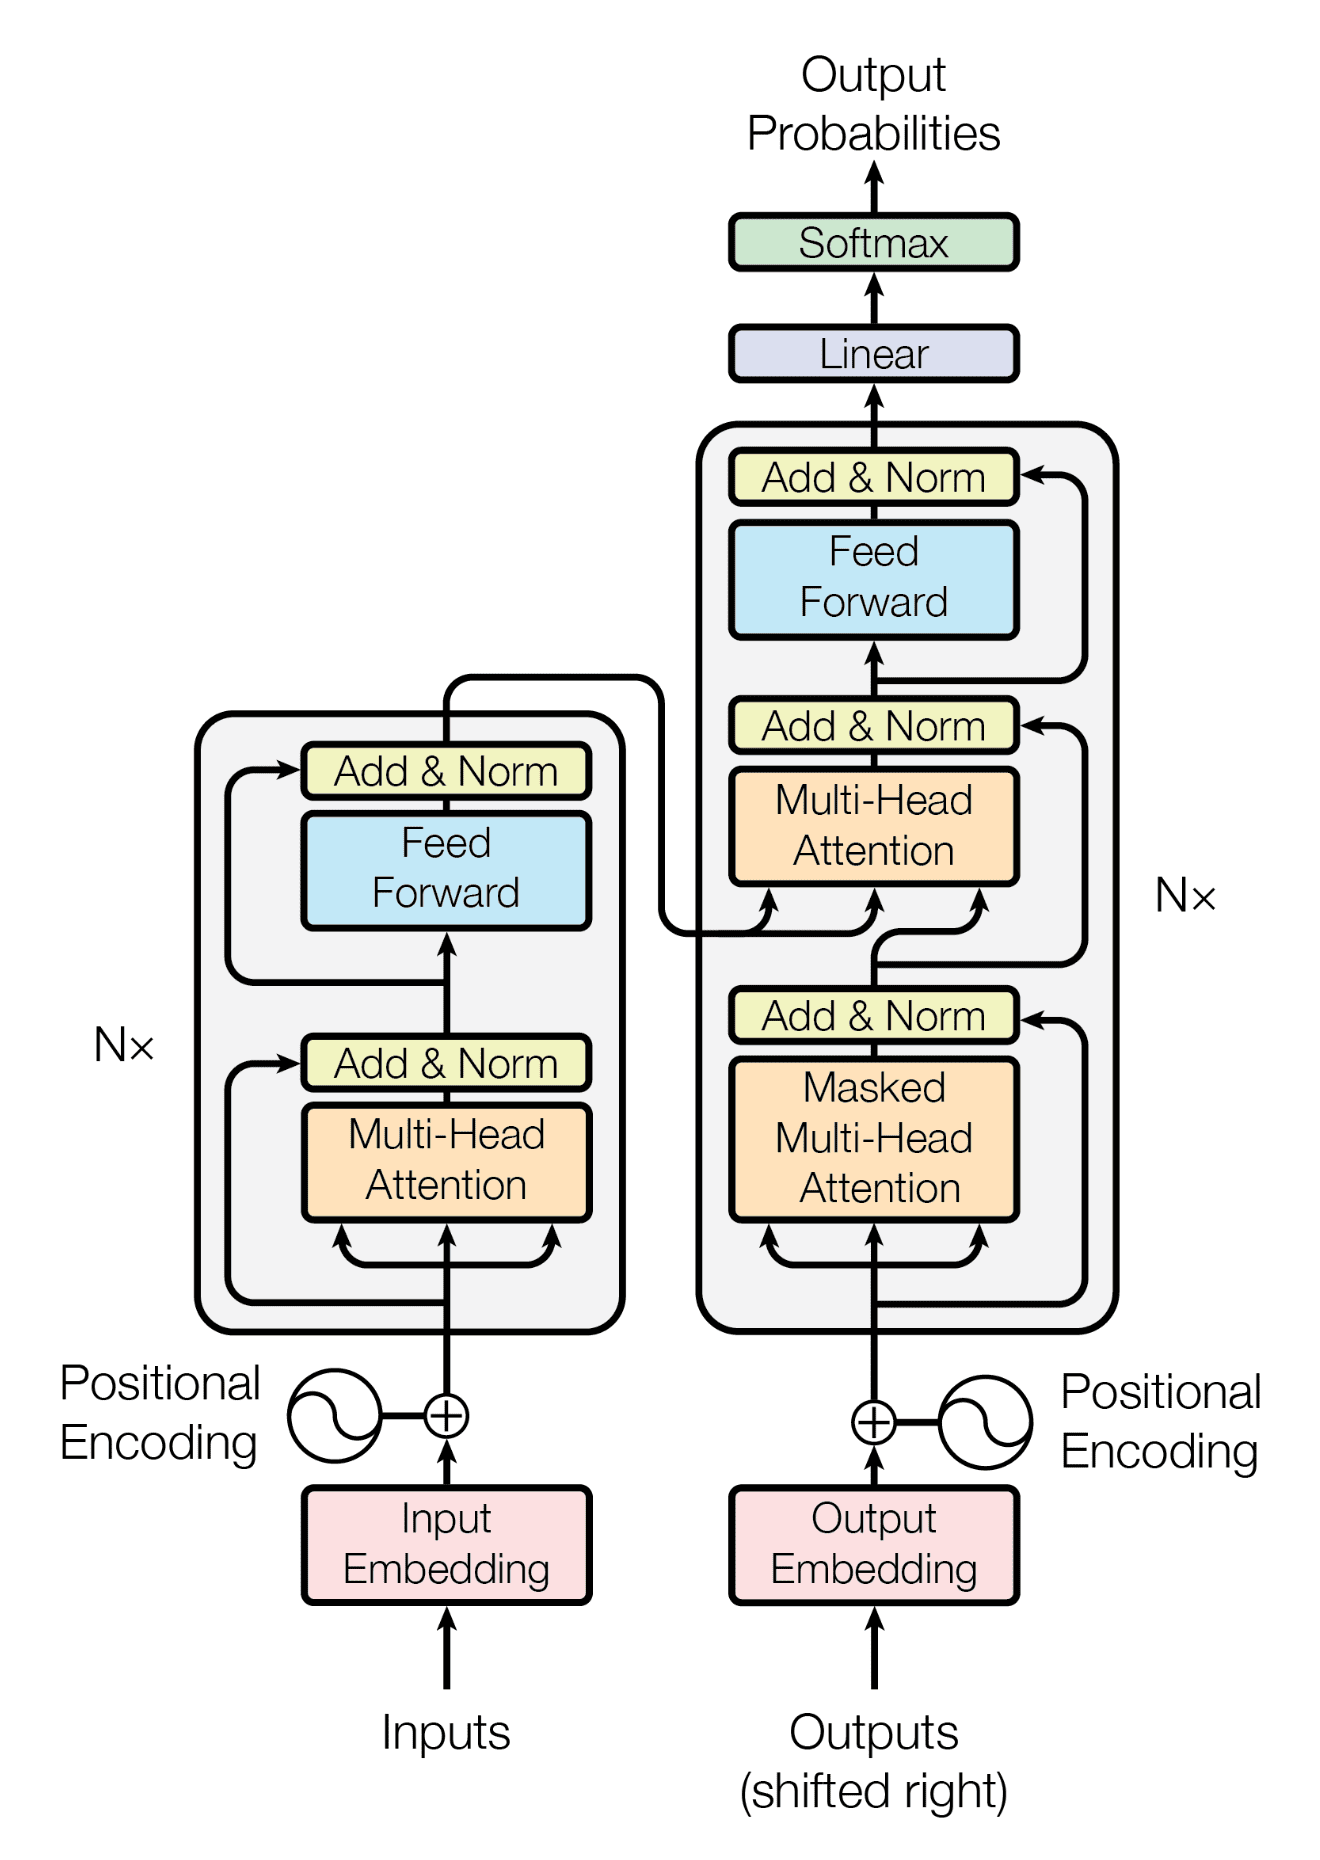
\includegraphics[scale=0.25]{images/attention-is-all-you-need}
        \caption{Tổng quan kiến trúc của \textit{Transformer}}
        \label{fig:attetion-is-all-you-need}
    \end{center}
\end{figure}

Nhờ không sử dụng kiến trúc hồi quy, \textit{Transformer} tránh được nhược điểm chí mạng của các mô hình loại này. Dựa hoàn toàn vào cơ chế \textit{attention}, cụ thể hơn là giới thiệu kiến trúc \textit{Hultihead attention} giúp việc song song tính toán mô hình. Từ đó mà tăng độ hiệu quả huấn luyện cũng như hiệu quả tính toán.

\section{Tokenization \& Word Embeddings}

Trong bài toán dịch máy, các đoạn văn bản thô cần phải được tiền xử lý, chuyển đổi thành các dạng dữ liệu mà máy tính có thể hiểu được. Quá trình đó được thực hiện như sau:
\begin{itemize}
	\item \textit{Tokenization} là quá trình tách đoạn văn bản ra thành các từ thành phần (\textit{token}). Các token này đã được quy định sẵn trong một tập các từ đã biết trước được gọi là kho từ vựng (\textit{vocabulary}). Với các từ lạ, không thuộc trong kho từ vựng sẽ được đánh dấu là \textit{<unk> (unknown)}.
	\item Các \textit{token} sau khi được tách ra vẫn chưa thể đưa vào mô hình do chúng vẫn ở dạng dữ liệu mà các mô hình chưa thể hiểu. Do đó, với mỗi \textit{token}, ta cần chuyển chúng thành các vector N chiều (N chọn trước) mang tính chất và đại diện cho từ đó. Với mỗi chiều của vector được biểu diễn bằng một số thực. Các vector này được gọi là các \textit{Word Embeddings}. Các \textit{Word Embeddings} sẽ là đầu vào của mô hình. Một số phương pháp để tính toán các \textit{Word Embeddings} trước đây gồm: \textit{CBOW, N-gram, skip-gram,...}
\end{itemize}

\begin{figure}[H]
    \begin{center}
        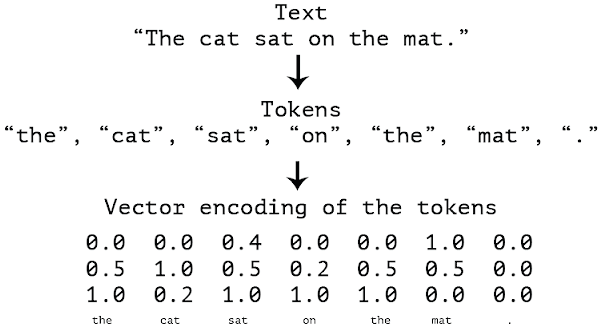
\includegraphics[scale=0.8]{images/token-embeddings}
        \caption{Tokenization \& word embeddings}
        \label{fig:token-embeddings}
    \end{center}
\end{figure}


\section{Graph Convolution Network (GCN)}
Khai thác quan hệ giữa các điểm dữ liệu với nhau là một đề tài được nhiều sự quan tâm trong học máy. Trong các mô hình học sâu trước đây, ta chỉ có thể trích xuất được các mối quan hệ thông thường từ các bộ dữ liệu \textit{Euclidian}.

\begin{figure}[H]
    \begin{center}
        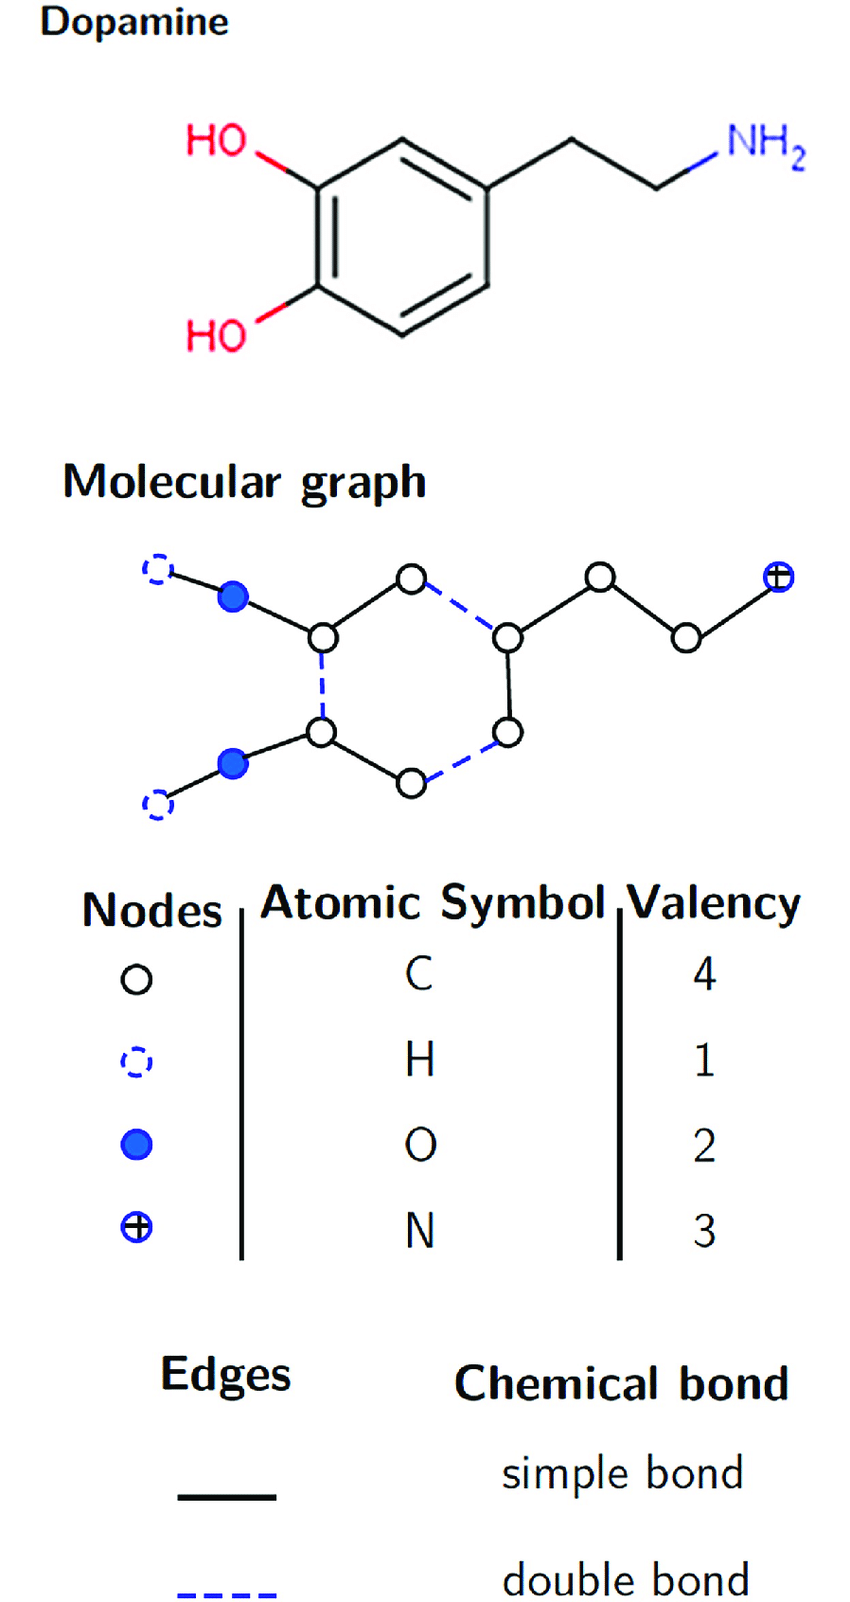
\includegraphics[scale=0.3]{images/chemistry-molecule}
        \caption{Các phân tử hóa học được biểu diễn dưới dạng đồ thị}
        \label{fig:chemistry-molecule}
    \end{center}
\end{figure}

Trong thực tế, không phải mọi dữ liệu đều biểu diễn ở dạng \textit{Euclidian}. Do đó, để khai thác được thông tin từ các bộ dữ liệu đồ thị (\textit{non-Euclidian}), ta cần sử dụng các mô hình \textit{Graph Neural Network (GNN)}. Trong vài năm qua, nhiều biến thể của GNN đã được phát triển. Trong đó, \textit{Graph Convolution Network (GCN)} là một biến thể quan trọng được xem như là biến thể cơ bản nhất của \textit{Graph Neural Network(GNN)}.

\textit{Graph Convolutional Network} ứng dụng phép tích chập được giới thiệu trong \textit{convolution layer} của \textit{mạng tích chập(CNN)}:
\begin{itemize}
	\item Đối với phép tích chập trên \textit{CNN}, một đoạn dữ liệu của lớp hiện tại sẽ được nhân vô hướng (tích chập) với một bộ lọc (\textit{filter} hoặc \textit{kernel}). Bộ lọc sẽ trượt trên bộ dữ liệu và các đầu ra của phép tích chập sẽ được truyền vào lớp tiếp theo của mạng.
	\item Với phép tích chập trên \textit{GCN}. Ta xét từng nút(\textit{node}) của đồ thị. Với mỗi nút, ta nhóm nút này với các nút kề của chính nó lại và thực hiền phép tích chập tương tự với một màn lọc. Do số lượng nút kề của mỗi nút là khác nhau, nên kích thước của \textit{filter} sẽ không cố định. Phép tích chập sẽ được thực hiện trên tất cả các nút của đồ thị.
\end{itemize}

\begin{figure}[H]
    \begin{center}
        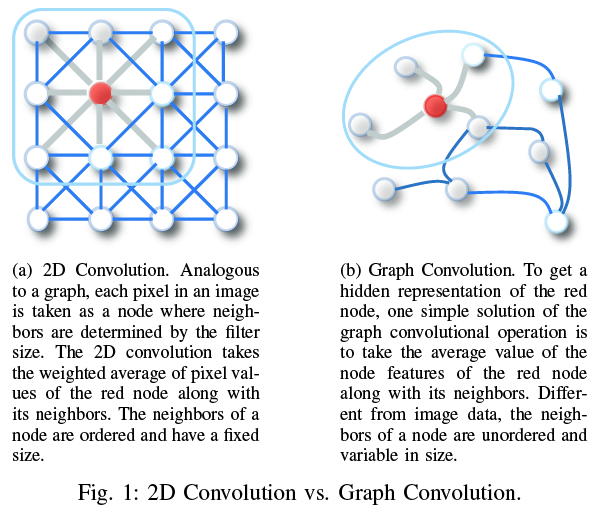
\includegraphics[scale=0.6]{images/cnn-vs-gcn}
        \caption{So sánh \textit{CNN} và \textit{GCN}}
        \label{fig:cnn-vs-gcn}
    \end{center}
\end{figure}

Nhận xét về phép tích chập 2 chiều của mô hình \textit{CNN}. Nếu ta xem mỗi điểm dữ liệu là một đỉnh của đồ thị và các điểm dữ liệu xung quanh sẽ có cạnh nối đến với đỉnh tương ứng. Phép tích chập của \textit{CNN} có ý nghĩa hoàn toàn giống với phép tích chập của mô hình GCN.


\section{WordGCN}
Quan hệ của các từ trong một ngôn ngữ là dạng quan hệ non-Euclidian. Do đó, trích xuất thông tin của chúng bằng các mô hình \textit{GCN} được kì vọng là có kết quả tốt hơn các phương pháp trước đó. Các loại thông tin có thể khai thác bao gồm: 
\begin{itemize}
	\item Thông tin về cú pháp (\textit{syntactic context}) của ngôn ngữ. Các từ trong một câu sẽ có các quy định về các mối quan hệ của chúng trong câu. Biểu diễn các mối quan hệ này là các cạnh còn các từ trong câu là các nút của đồ thị. Từ đó mà ta có thể khai thác được các đặc trưng cú pháp của các từ. Mô hình \textit{SynGCN} sẽ giúp ta huấn luyện được các \textit{embeddings} mang các thông tin trên.

    \begin{figure}[H]
        \begin{center}
            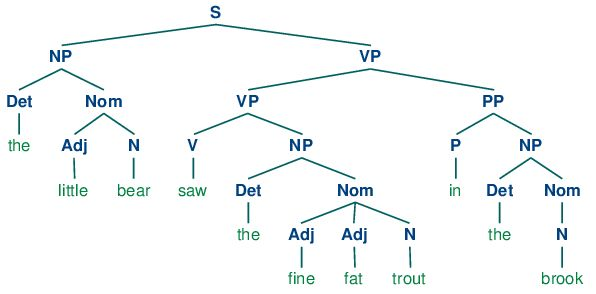
\includegraphics[scale=0.8]{images/syntactic-context}
            \caption{Thông tin cú pháp của một câu được biểu diễn dưới dạng đồ thị}
            \label{fig:syntactic-context}
        \end{center}
    \end{figure}

	\item Thông tin về ngữ nghĩa (\textit{semantic context}) của ngôn ngữ. Ý nghĩa của các từ sẽ có các quan hệ với nhau như: đồng nghĩa, trái nghĩa, kế thừa,... Nhờ các mối quan hệ đó, ta có thể biểu diễn được đồ thị ngữ nghĩa của các từ trong bộ từ vựng. Từ đó mà ta có thể khai thác được các đặc trưng ngữ nghĩa của các từ. Mô hình \textit{SemGCN} sẽ giúp ta huấn luyện được các \textit{embeddings} mang thông tin ngữ nghĩa.

    \begin{figure}[H]
        \begin{center}
            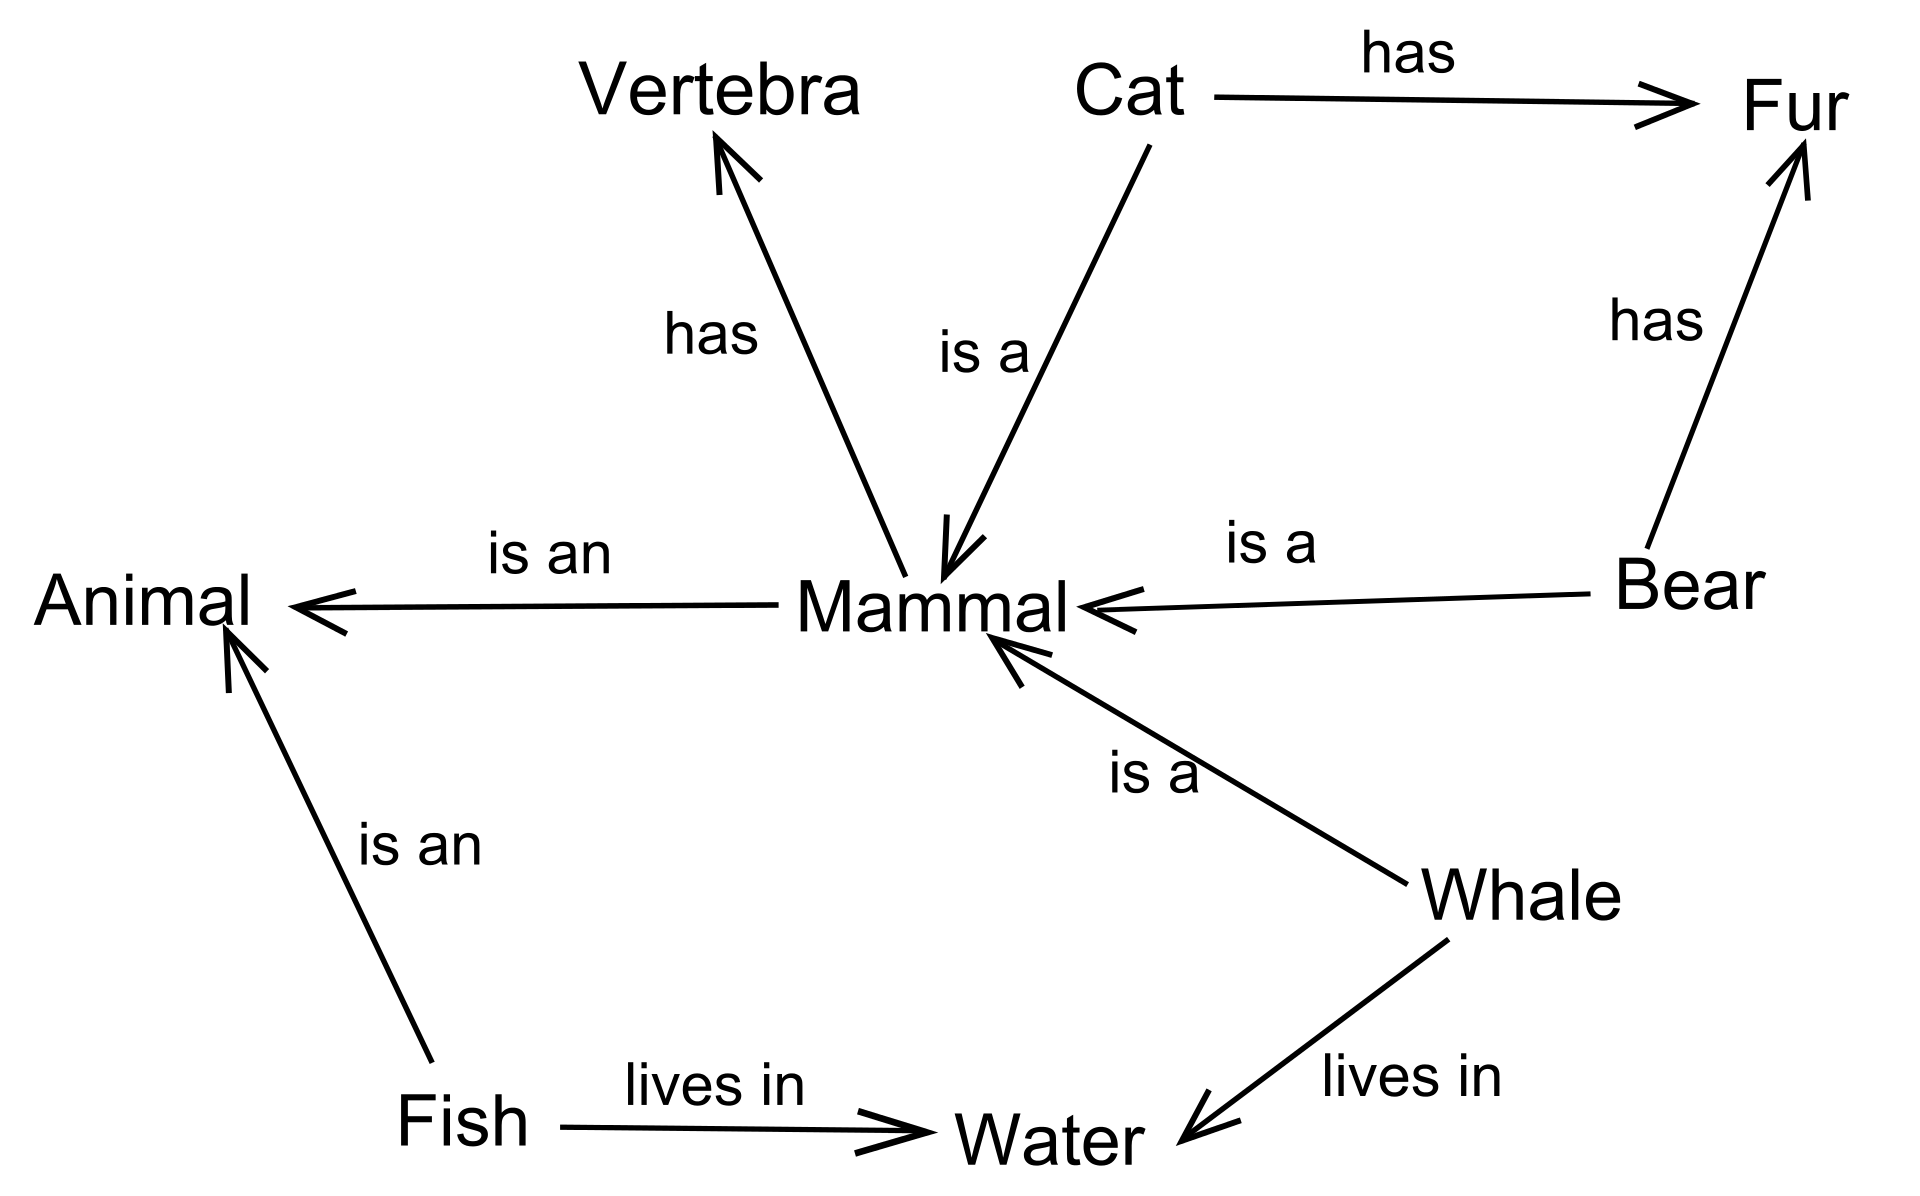
\includegraphics[scale=0.2]{images/semantic-context}
            \caption{Thông tin ngữ nghĩa của các từ được biểu diễn dưới dạng đồ thị}
            \label{fig:semantic-context}
        \end{center}
    \end{figure}

\end{itemize}

\chapter{Tổng quan lý thuyết}
\label{Chapter2}
\section{Mô hình transformer dịch máy}

\subsection{Tổng quan mô hình}

 \textit{Transformer}  là một mô hình có kiến trúc \textit{Encoder-Decoder}. Mô hình bao gồm 2 thành phần chính là \textit{Encoder (bộ mã hóa)} và \textit{Decoder(bộ giải mã)}. Khi đưa một đoạn văn bản nguồn vào, mô hình sẽ xử lý vào đưa ra đoạn văn bản có ngữ nghĩa tương ứng ở ngôn ngữ đích.

\begin{figure}[H]
    \begin{center}
        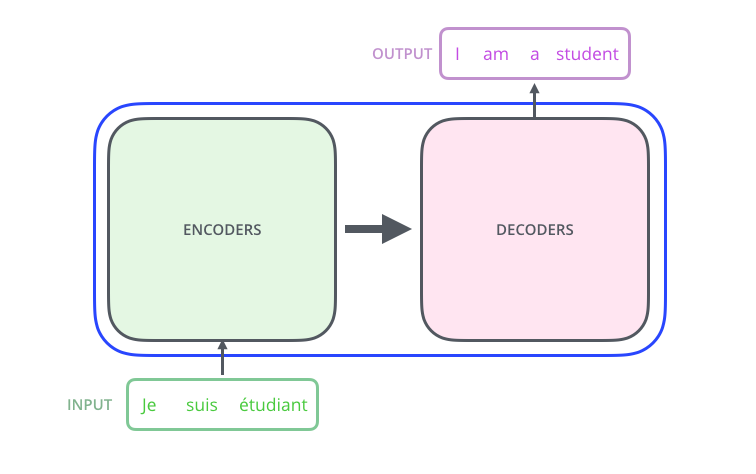
\includegraphics[scale=0.4]{images/The_transformer_encoders_decoders}
        \caption{Minh họa kiến trúc Encoder-Eecoder \cite{illustrated.transformer}}
        \label{fig:encoder-decoder}
    \end{center}
\end{figure}

Cụ thể hơn, Bộ mã hóa sẽ bao gồm nhiều lớp mã hóa xếp chồng lên nhau. Theo \cite{transformer}, họ sử dụng 6 lớp mã hóa để tạo thành một bộ mã hóa.  Bộ giải mã, tương tự cũng được xếp chồng bởi các lớp giải mã. Số lượng lớp của 2 thành phần phải bằng nhau.

\begin{figure}[H]
    \begin{center}
        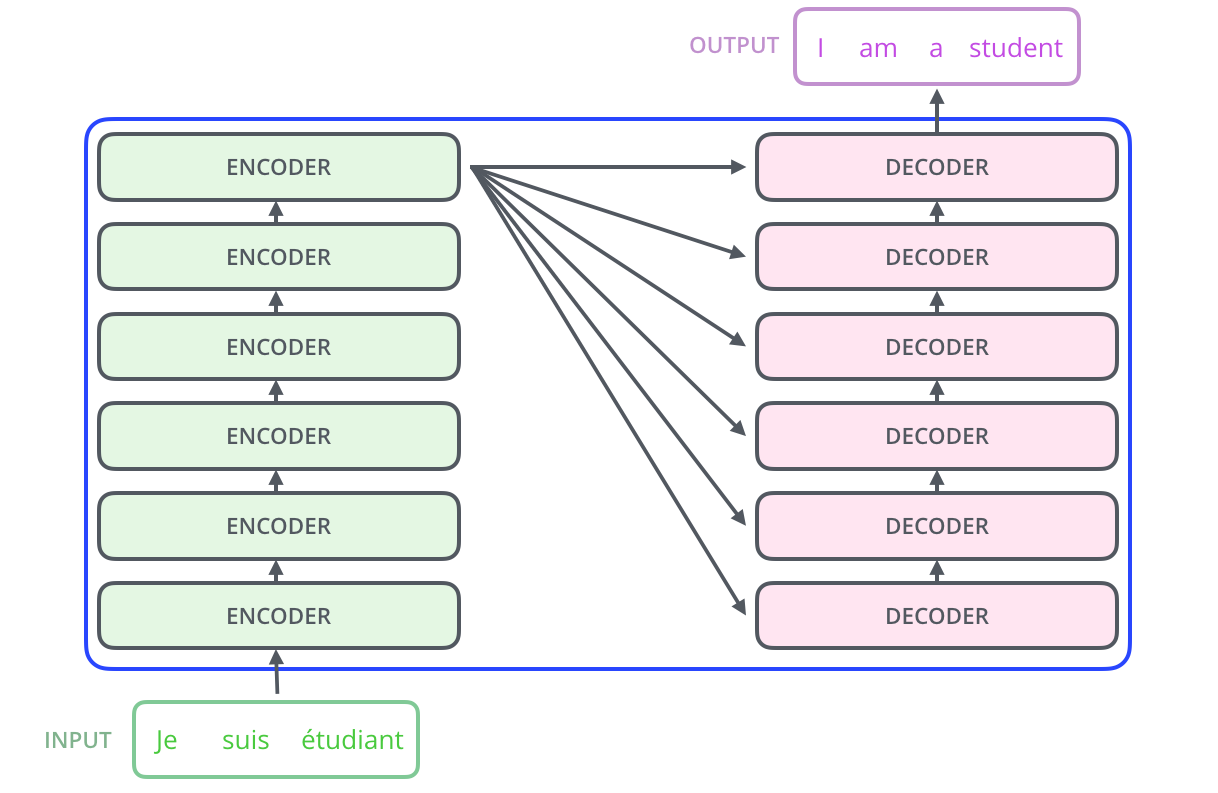
\includegraphics[scale=0.35]{images/The_transformer_encoder_decoder_stack}
        \caption{\textit{Bộ mã hóa} và \textit{bộ giải mã} trong \textit{Transformer}\cite{illustrated.transformer}}
        \label{fig:encoder-decoder-stack}
    \end{center}
\end{figure}



\subsection{Lớp mã hóa (Encoder)}
Các lớp của bộ mã hóa là độc lập nhau và có cấu trúc tương tự nhau. Đầu vào của lớp đầu tiên sẽ là các \textit{word embeddings} đã được xử lý qua lớp \textit{positional encoding}, các lớp phía trên sẽ có đầu vào là các vector đầu ra từ lớp ngay dưới. Các vector đầu vào của các lớp này được gọi là \textit{context vector}.

Với mỗi lớp mã hóa sẽ bao gồm 2 lớp con:
\begin{itemize}
	\item \textit{Self-attetion}: Với mỗi từ trong đoạn văn bản, xem xét độ liên quan của nó với các từ khác trong câu đầu vào. Đưa ra phân bố xác xuất đối với từng từ một.
	\item \textit{Feed forwarding}: Mã hóa phân bố xác xuất tính toán được thành các context vector để đưa vào các lớp mã hóa phía trên.
\end{itemize}

\begin{figure}[H]
    \begin{center}
        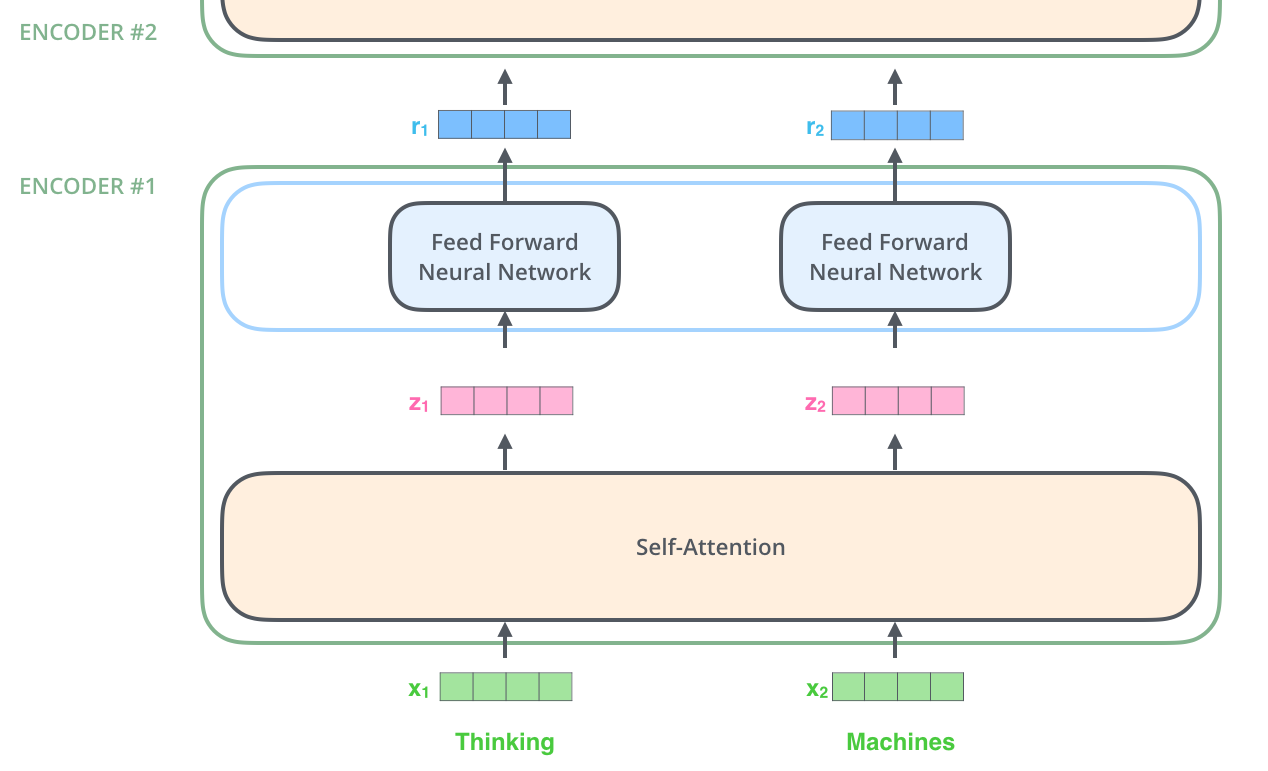
\includegraphics[scale=0.35]{images/encoder}
        \caption{Kiến trúc lớp mã hóa\cite{illustrated.transformer}}
        \label{fig:encoder}
    \end{center}
\end{figure}


\subsubsection{Cơ chế Self-attention}

\textit{Self-attention} là một cơ chế mới được giới thiệu trong \textbf{attention is all need} \cite{transformer}. Cơ chế này khác với cơ chế \textit{attention} trong các mạng \textit{Seq2Seq} trước đó. \textit{Self-attention} cho phép ta biểu diễn lại mối quan hệ giữa các từ trong một đoạn văn bản.

\begin{figure}[H]
    \begin{center}
        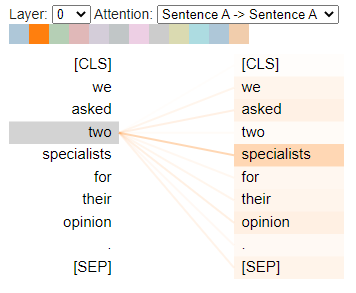
\includegraphics[scale=1.0]{images/self-attention}
        \caption{Minh họa cơ chế \textit{Self-attention}\cite{illustrated.transformer}}
        \label{fig:self-attention}
    \end{center}
\end{figure}

Hình trên cho ta một minh họa về cơ chế \textit{self-attention}. Xét từ \textit{"two"}, theo tư duy của con người, ta sẽ phân tích xem từ "two" trong câu đang có quan hệ gì với những từ khác. Ngoài ra, ta còn xem xét tầm quan trọng của các từ khác tác động lên ý nghĩa của câu. Từ đó mà ta có thể có được một cái nhìn rõ ràng hơn về vai trò của từ này trong câu.

Cụ thể hơn, khi mô hình xử lý từ \textit{"two"}, \textit{self-attention} cho ta thấy được mối liên kết của nó với từ \textit{"specialists"}. Thể hiện vai trò của nó là dùng để chỉ số lượng của các chuyên gia là hai.

Việc tính toán ở mỗi lớp \textit{Self-attention} được tính toán dựa trên công thức sau:

\begin{equation*}
	Attention = Softmax(\frac{QK^T}{\sqrt{d}})V
\end{equation*}

Trong đó, các ma trận $Q, K, V$ lần lượt là các ma trận \textit{Query, Key, Value}. Hai ma trận $Q$ và $K$ được dùng để tính toán mối quan hệ giữa các từ trong câu. Còn mỗi dòng thứ của ma trận $V$ đại diện cho từ thứ $i$ trong câu. Từ phân bố \textit{softmax}, ta tính được \textit{context vector}, tổng hợp được các thông tin của từ hiện tại và các từ liên quan đến nó. 

Trong công thức, ta thấy được tích vô hướng của ma trận $Q$ và $K$ được chuẩn hóa bởi hệ số $\sqrt{d}$ ($d$ là số chiều của \textit{vector embedding}). Lý do cho việc chuẩn hóa này là do khi $d$ có giá trị lớn, tích vô hướng của $Q$ và $K$ sẽ có giá trị lớn theo do đó, nếu không chuẩn hóa về giá trị nhỏ hơn thì hàm \textit{softmax} sẽ có độ hội tụ khá chậm

\begin{figure}[H]
    \begin{center}
        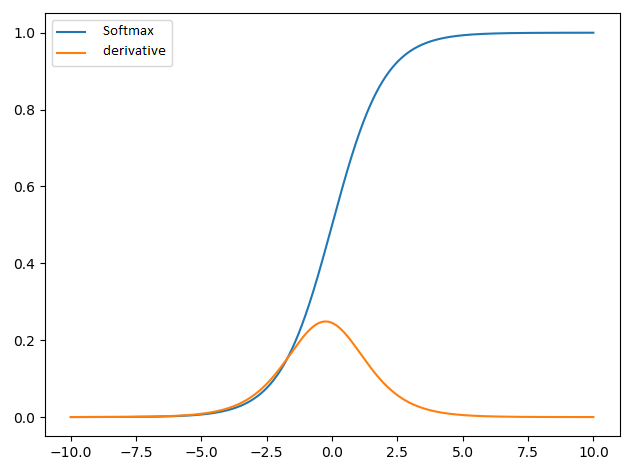
\includegraphics[scale=0.7]{images/softmax-func}
        \caption{Đồ thị hàm \textit{softmax} và đạo hàm của một thành phần trong tập phân loại}
        \label{fig:softmax-func}
    \end{center}
\end{figure}


\begin{algorithm}[H]
    \caption{Self\_attention($context, w_K, w_Q, w_V$)}
    \begin{algorithmic}[1]
		\State \textbf{Result:} $Z$
		\State {$K \gets context \times w_K$}
		\State {$Q \gets context \times w_Q$}
		\State {$V \gets context \times w_V$}
		\State {$Score \gets QK^T$}
		\State {$Z \gets \frac{softmax(Score)}{\sqrt{d}}V$}
    \end{algorithmic}
\end{algorithm}

Từ công thức tính của \textit{self-attention}, ta có thể thấy rõ sự khác biệt giữa bộ mã hóa của \textit{transformer} và bộ mã hóa của các mô hình \textit{Seq2Seq} sử dụng mạng hồi quy. Đối với mô hình hồi quy, dữ liệu đầu vào phải được mã hóa một cách tuần tự. Trong khi đối với \textit{self-attention}, các từ trong văn bản có thể được mã hóa một cái song song và không bị phụ thuộc vào nhau. Nhờ đó mà có thể tăng được hiệu quả tính toán.

\subsubsection{Cơ chế Multihead-attention}
Đầu ra của \textit{self-attention} cho ta biết được mối quan hệ của các từ trong câu dựa trên một góc nhìn nào đó. Bằng các xếp chồng nhiều lớp \textit{self-attention} lại với nhau. Ta có thể biết được sự liên quan của các từ ngữ trong câu với nhiều gốc nhìn khác nhau. Từ đó mà có được thông tin đầy đủ hơn về câu cần dịch. 

Cơ chế xếp chồng nhiều lớp \textit{self-attention} lại với nhau được gọi là \textit{Multihead attention}. 

Ngoài ra, sử dụng cơ chế \textit{self-attention} còn giúp ta tránh được trường hợp một từ phụ thuộc hoàn toàn vào chính nó. Ta mong muốn một phân bố xác suất quan hệ giữa một từ với các từ có ảnh hưởng đến nó.

Với việc sử dụng N lớp \textit{self-attention} chạy song song với các bộ trọng số khác nhau, ta có được N ma trận \textit{context} khác nhau. Lúc này, ta cần có một phương phát khác để tổng hợp thông tin từ các lớp \textit{self-attention} này lại để đưa vào lớp \textit{feed-forward}. 

\begin{figure}[H]
    \begin{center}
        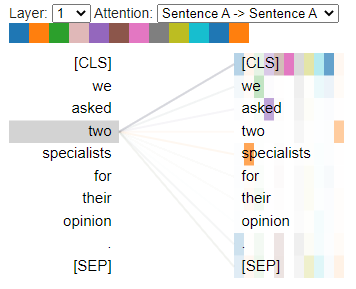
\includegraphics[scale=0.8]{images/multihead-context-vector}
        \caption{Minh họa cơ chế \textit{Multihead attention}}
        \label{fig:multihead-context-vector}
    \end{center}
\end{figure}

Để làm được việc đó, \textit{Transformer} ghép theo chiều ngang các ma trận \textit{context} lại rồi nhân với một bộ trọng số để đưa ra một kết quả duy nhất là một ma trận với các dòng là các \textit{context vector} cũng đồng thời là đầu vào cho bộ giải mã ở phía trên.

\begin{figure}[H]
    \begin{center}
        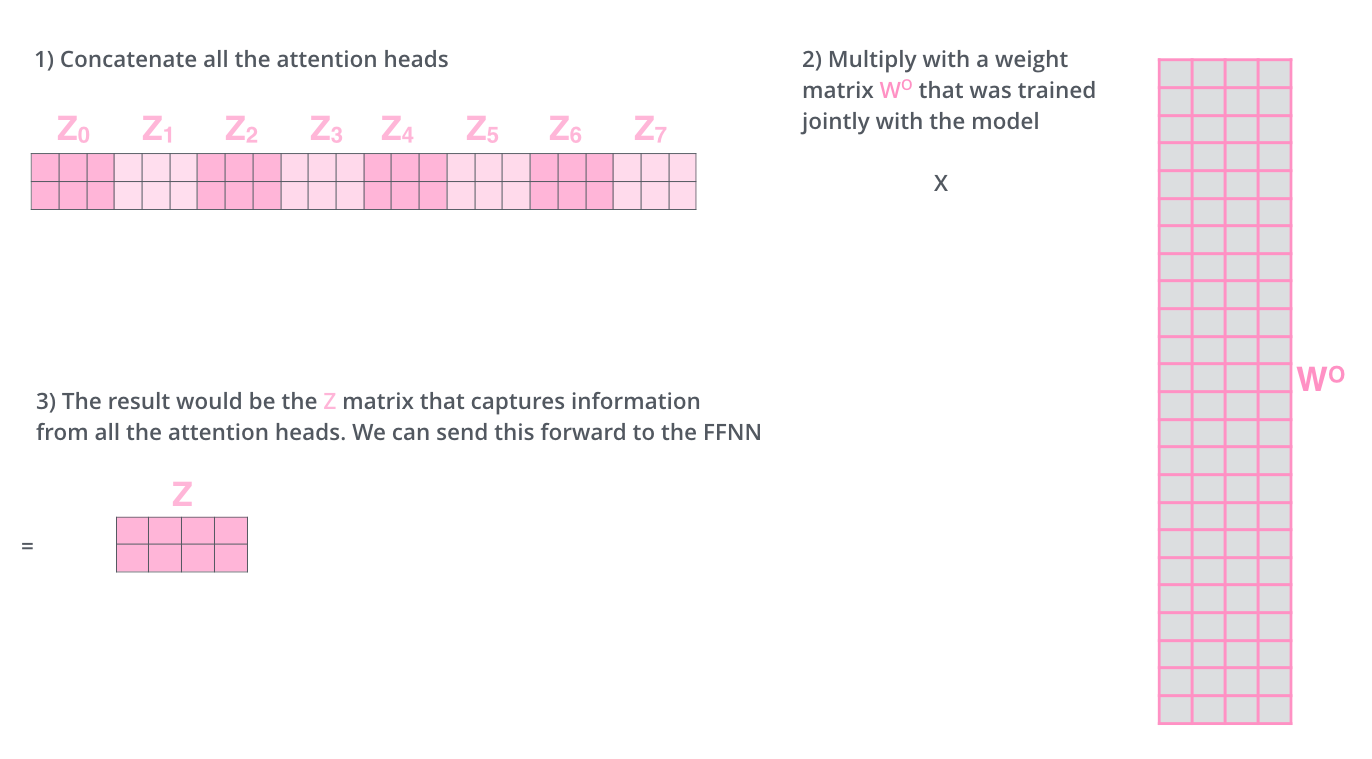
\includegraphics[scale=0.3]{images/transformer_attention_heads_weight_matrix_o}
        \caption{Cơ chế tổng hợp feed-forward trong Multihead attention\cite{illustrated.transformer}}
        \label{fig:multihead-feed-forward}
    \end{center}
\end{figure}

Hình dưới minh họa cho việc sử dụng nhiều lớp \textit{self-attention} trên cùng một câu với mỗi một màu tương ứng với kết quả của một lớp \textit{self-attention} khác nhau.

\begin{algorithm}[H]
    \caption{Multihead attention($context$)}
    \begin{algorithmic}[1]
		\State \textbf{Result:} $Z \times w_O$
		\For{$1...\#head$}
			\State $Z_i \gets self\_attention(context, wK_i, wQ_i, wV_i)$
		\EndFor
		\State $Z \gets [Z_1, Z_2,... ,Z_{\#head}]$
    \end{algorithmic}
\end{algorithm}

\begin{figure}[H]
    \begin{center}
        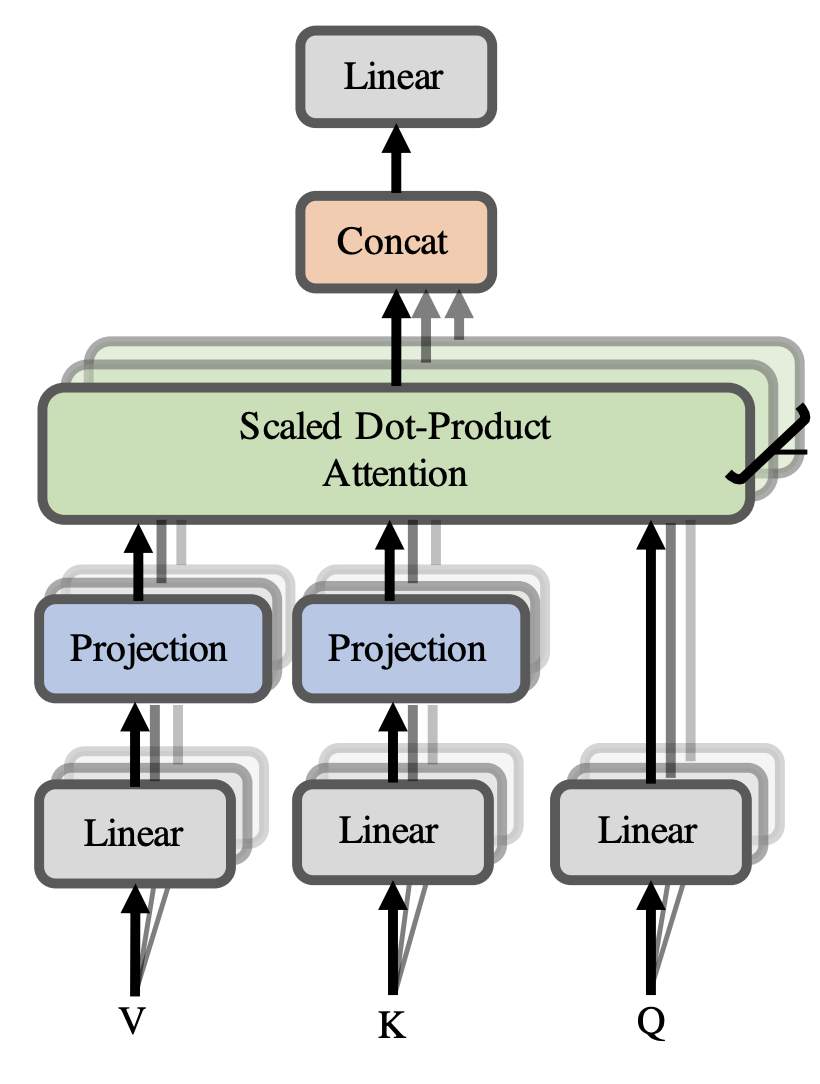
\includegraphics[scale=0.6]{images/multihead-attention}
        \caption{Minh họa kiến trúc của \textit{Multihead attention}\cite{lil.transformer}}
        \label{fig:multihead-attention}
    \end{center}
\end{figure}

\subsubsection{Positional encoding}

Cách tính toán song song của cơ chế \textit{self-attention} dẫn đến một vấn đề đối với các từ trong đầu vào. \textit{Embeedings} biểu diễn các từ này chưa biểu diễn được thông tin về thứ tự của các từ trong câu. Trong khi thông tin này là một thông tin quan trọng vì thay đổi vị trí của các từ có thể dẫn đến một câu hoàn toàn khác ý nghĩa.

Một ví dụ về việc đối chỗ một từ trong câu khiến cho ý nghĩa của câu trở nên trái ngược hoàn toàn:
\begin{itemize}
	\item "Please don't go! I love you!"
	\item "Please go! I don't love you!"
\end{itemize}

 \textit{Transformer}  sử dụng cơ chế \textit{positional encoding}. Cơ chế này giúp đưa thông tin về vị trí của các từ vào trong các \textit{embeddings}. Cụ thể hơn, trước khi \textit{embeddings} được đưa vào trong mô hình, nó được cộng với một vector tương ứng với vị trí trong câu. Những vector này tuân theo một một quy định nhất định. Chúng phải thể hiện được sự khác biệt về vị trí của các từ trong câu và cả khoảng cách của các từ trong câu. 

Công thức tính toán các vector này như sau: 
\begin{equation*}
	PE_{(pos, 2i)} = \sin{\frac{pos}{10000^{\frac{2i}{d_model}}}}
\end{equation*}
\begin{equation*}
	PE_{(pos, 2i+1)} = \cos{\frac{pos}{10000^{\frac{2i}{d_model}}}}
\end{equation*}

\begin{figure}[H]
    \begin{center}
        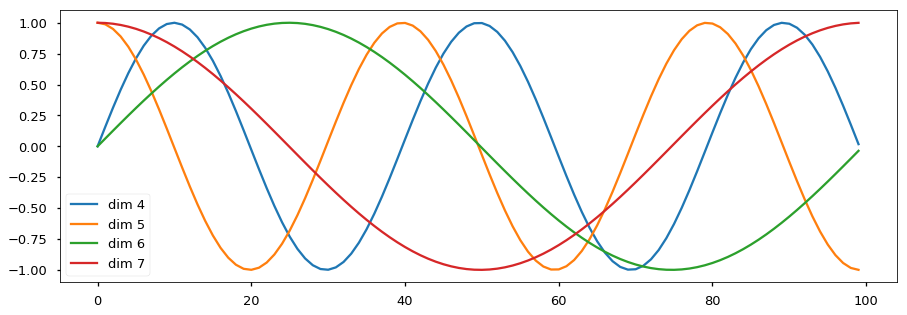
\includegraphics[scale=0.5]{images/positional-embedding}
        \caption{Đồ thị positional embedding \cite{annotated.transformer}}
        \label{fig:positional embedding}
    \end{center}
\end{figure}



\subsection{Lớp giải mã}
Các lớp của bộ giải mã cũng có 2 lớp con là \textit{Self-attention} và \textit{Feed-forwarding} giống với bộ mã hóa. Tuy nhiên giữa 2 lớp con này có một lớp trung gian là \textit{Encoder-Decoder attention}. Lớp này có cơ chế giống với cơ chế \textit{attention} trong mô hình \textit{Seq2Seq} với thông tin của các \textit{lớp ẩn (hidden layers)} chính là đầu ra của bộ mã hóa.

\begin{figure}[H]
    \begin{center}
        \includegraphics[scale=0.5]{images/transformer_decoder}
        \caption{Minh họa kiến trúc bộ lớp mã hóa \cite{illustrated.transformer}}
        \label{fig:decoder}
    \end{center}
\end{figure}

\subsubsection{Masked self attention}

Khác với lớp \textit{self-attention} ở bộ mã hóa, lớp \textit{masked self attention} ở bộ giải mã chỉ tìm kiếm các mối quan hệ của từ hiện tại với các từ đã được giải mã trước đó. Do đó, trước khi thực hiện tính toán trên hàm \textit{softmax}, giá trị \textit{score} của các từ chưa được giải mã sẽ được gắn nhãn là $-\infty$. Sau đó, các bước tính toán sẽ tương tự như trong bộ mã hóa.

\begin{figure}[H]
    \begin{center}
        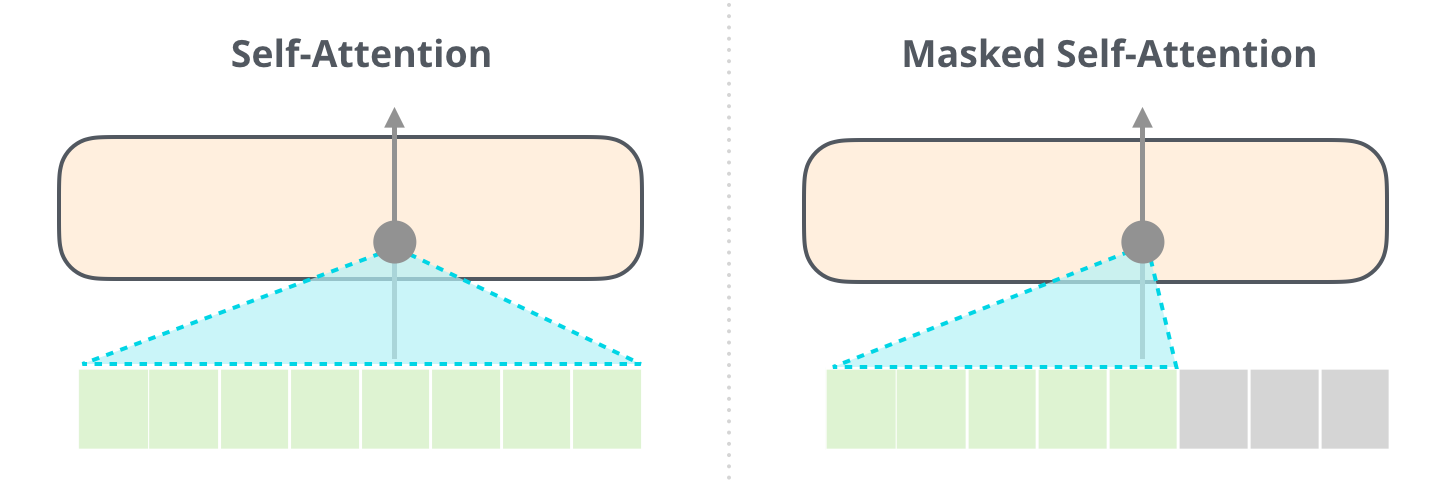
\includegraphics[scale=0.3]{images/self-attention-and-masked-self-attention}
        \caption{So sánh \textit{self attention} và \textit{maked self attention}}
        \label{fig:masked-self-attention}
    \end{center}
\end{figure}

Ta có thể điều chỉnh lại hàm \textit{self attention} như sau:

\begin{algorithm}[H]
    \caption{Self\_attention($context, w_K, w_Q, w_V, masked$)}
    \begin{algorithmic}[1]
		\State \textbf{Result:} $Z$
		\State {$K \gets context \times w_K$}
		\State {$Q \gets context \times w_Q$}
		\State {$V \gets context \times w_V$}
		\State {$Score \gets QK^T$}
		\For{$i=masked + 1...len(context)$}
			\State Cột thứ i của $Score = -\infty$
		\EndFor
		\State {$Z \gets \frac{softmax(Score)}{\sqrt{d}}V$}
    \end{algorithmic}
\end{algorithm}

Tham số \textit{masked} thể hiện kể từ vị trí này, các phần tử phía sau của \textit{score} sẽ được gán giá trị $-\infty$. Hàm \textit{self\_attention} được gọi bởi hàm \textit{multihead\_attention}. Do đó, ta cần truyền thêm tham số masked vào hàm này. Ta mặc định \textit{masked = len(context)}, nhờ vậy mà mà cần truyền thêm tham số này khi gọi trong bộ mã hóa.


\subsubsection{encoder-decoder attention}
Một điểm khác biệt dễ thấy giữa bộ mã hóa và bộ giải mà là lớp \textit{encoder-decoder attention} được đặt giữa 2 lớp \textit{self attetion} và \textit{feed-forward}. Công dụng của lớp này giúp cho lớp giải mã có thể giải mã ra được các từ của văn bản đích dựa trên độ liên quan của mỗi từ với các từ trong văn bản nguồn. 

\begin{figure}[H]
    \begin{center}
        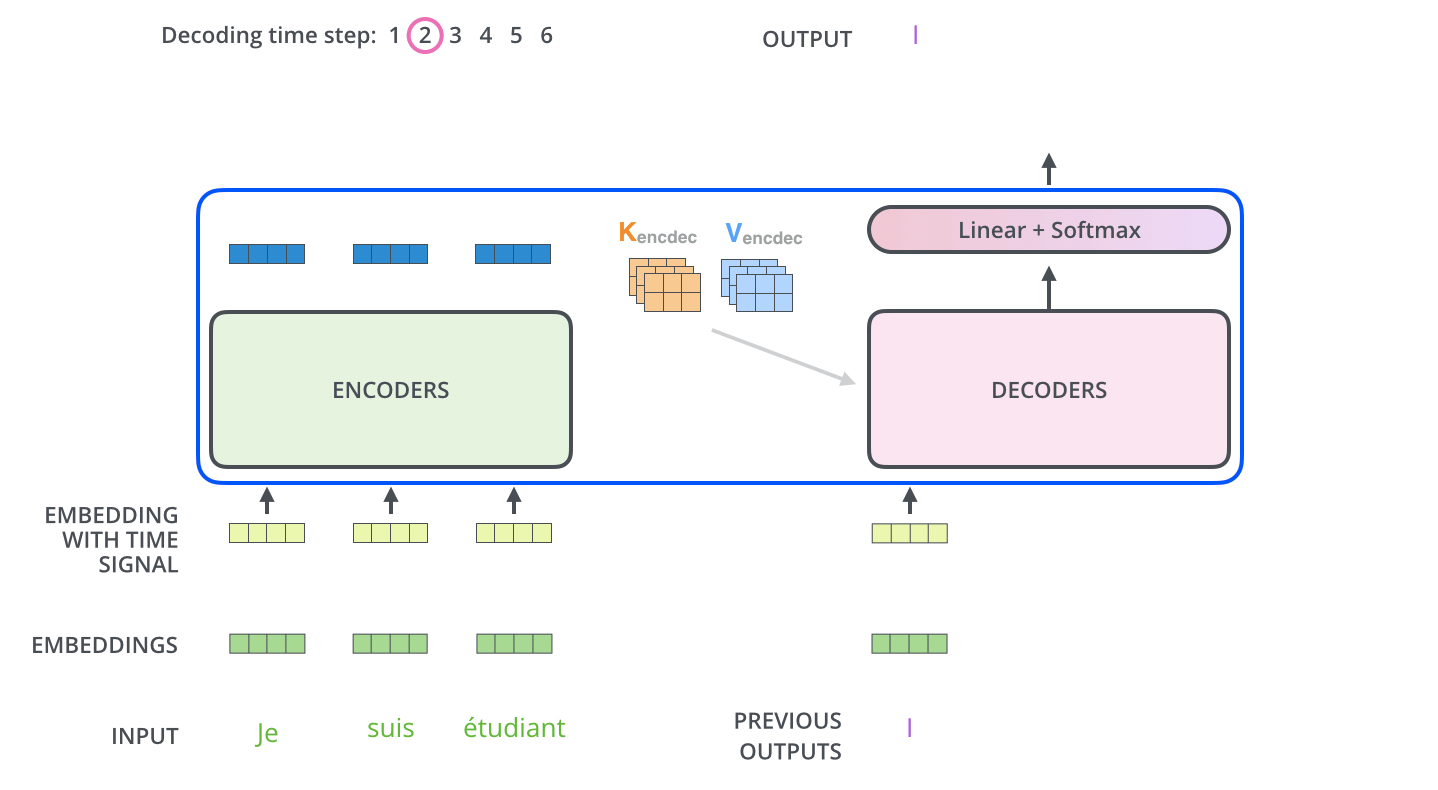
\includegraphics[scale=0.41]{images/encoder-decoder-attention}
        \caption{Minh họa cơ chế \textit{encoder-decoder-atention} \cite{illustrated.transformer}}
        \label{fig:encoder-decoder-attention}
    \end{center}
\end{figure}

Đầu ra lớp trên cùng của mã hóa sẽ được biến đổi thành 2 vector K và V. Quá trình giải mã được thực hiện như sau:


\begin{algorithm}[H]
    \caption{decoder(context, pos)}
    \begin{algorithmic}[1]
		\State \textbf{Result:} $feed\_forward(context)$
		\State $context \gets multihead\_attention(context, masked = pos)$
		\State $context \gets normalize(context)$
		\State $context \gets encoder\_decoder\_attention(K_{enc}, V_{env}, context)$
    \end{algorithmic}
\end{algorithm}

Để biểu thị cho mở đầu của đoạn văn bản và kết thúc của đoạn văn bản đến đánh dấu việc bắt đầu giải mã và kết thúc giải mã.  \textit{transformer}  sử dụng 2 token đặc biệt nằm tách biệt với bộ từ vựng: \textit{<bos> (begin of sentence)} và \textit{<eos> (end of sentence)}.

Quá trình giải mã sẽ được bắt đầu với token \textit{<bos>} và thực hiện một cách tuần từ cho đến khi giải mã ra token \textit{<eos>}. Từ được giải mã ở bước trước sẽ được sử dụng làm đầu vào cho bước giải mã tiếp theo. Cụ thể thuật toán của toàn bộ quá trình giải mã như sau:

\begin{algorithm}[H]
    \caption{Quá trình giải mã}
    \begin{algorithmic}[1]
		\State Khởi tạo $output_i \gets <bos>$
		\State Khởi tạo $i \gets 1$
		\Do
			\State $embed_i \gets position\_encoding(output_{i-1})$
			\State $context \gets embed_i$
			\For $j = 1...\#layer$
				\State $context \gets decoder(context, masked = i)$
			\EndFor
			\State $output_i \gets softmax(context)$
		\doWhile $output_i \neq <eos>$
    \end{algorithmic}
\end{algorithm}


\subsection{residuals}
Để tránh các trường hợp \textit{Gradient biến mất},  \textit{Transformer}  kết hợp kiến trúc \textit{residual} vào các lớp mã hóa. Từ đó mà thông tin từ các lớp trước có thể được sử dụng lại trong khi huấn luyện các lớp sau.

với mỗi lớp con trong cả bộ mã hóa lẫn bộ giải mã, ta đặt thêm một lớp \textit{normalize} vào ngay trên lớp con đó. Lớp \textit{normalize} này nhận đầu vào là kết quả của lớp con ngay dưới của nó và cả đầu vào trước khi đi vào lớp con đó. Thưc hiện phép cộng hai ma trận này và chuẩn hóa lại trước khi đưa vào lớp con phía trên.

\begin{figure}[H]
    \begin{center}
        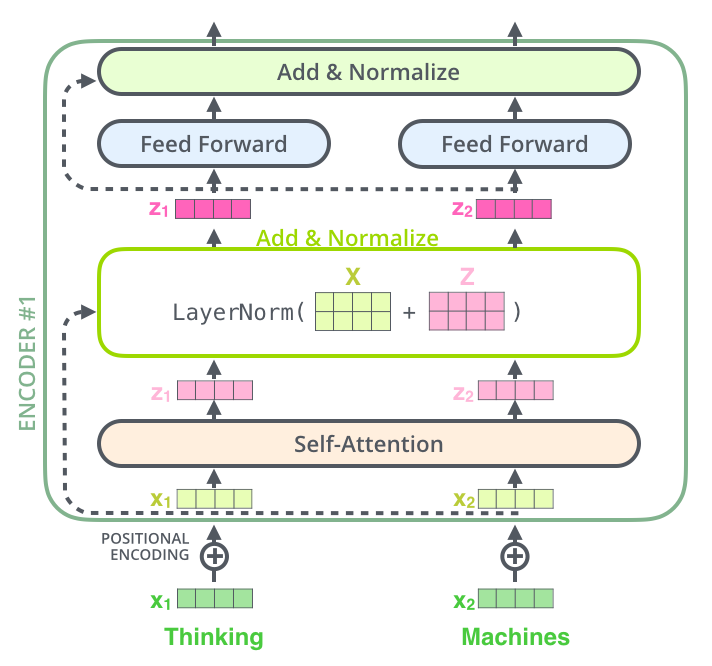
\includegraphics[scale=0.5]{images/residual}
        \caption{Minh họa kiến trúc \textit{residual}\cite{illustrated.transformer}}
        \label{fig:residual}
    \end{center}
\end{figure}


\subsection{Tổng kết mô hình}

Tổng kết lại, kiến trúc của \textit{Transformer} bao gồm 2 thành phần chính là bộ mã hóa và bộ giải mã. Bộ mã hóa được tạo bởi nhiều lớp con gọi là các lớp mã hóa. Tương tự, bộ giải mã cũng được hình thành từ các lớp giải mã được xếp chồng lên nhau. Số lượng lớp con của bộ mã hóa bằng với số lượng lớp con của bộ giải mã.

Với mỗi lớp con của bộ mã hóa sẽ bao gồm một lớp multihead-attention và một lớp feed-forward. Ngoài ra còn áp dụng thêm kiến trúc residual block với các lớp normalize.

Với mỗi lớp giải mã, chúng được xếp chồng bởi 3 lớp con lần lượt là: \textit{Masked Multihead Attention}, \textit{Encoder Decoder Attention} và \textit{Feed Forwarding}. Lớp giải mã cũng được áp dụng kiến trúc \textit{Residual block} giúp mô hình tránh được hiện tượng \textit{Gradient biến mất}

\begin{figure}[H]
    \begin{center}
        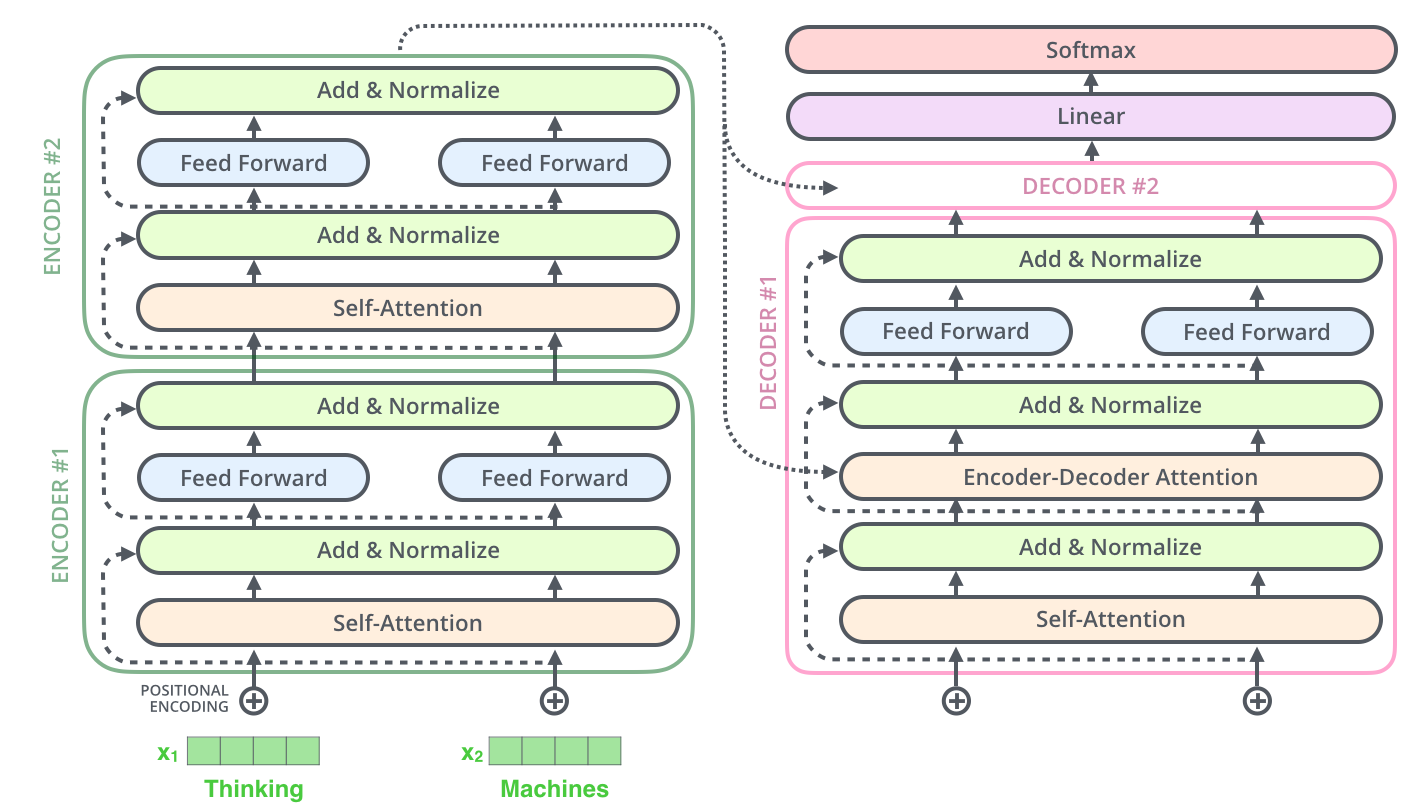
\includegraphics[scale=0.3]{images/transformer_sumary}
        \caption{Tổng kết mô hình \textit{Transformer} \cite{illustrated.transformer}}
        \label{fig:transformer-summary}
    \end{center}
\end{figure}


\section{Mô hình WordGCN huấn luyện word embeddings cho kho ngữ liệu}

\subsection{Lý thuyết đồ thị cơ bản}

\subsubsection{Định nghĩa đồ thị}

Đồ thị được định nghĩa là một cấu trúc rời rạc gồm các đỉnh và các cạnh nối các đỉnh đó. Ký hiệu biểu diễn một đồ thị như sau:
\begin{equation*}
	G = (V,E)
\end{equation*}

Trong đó, V là tập các \textit{đỉnh (Vertices)} và E là tập các \textit{cạnh (Edges)}. Các cạnh trong tập E được bởi diễn bởi một cặp (x,y) với $x,y \in V$. Số lượng đỉnh của đồ thị là $|V| = n$, còn số lượng cạnh của đồ thị là $|E| = m$

\subsubsection{Các loại đồ thị}
\textit{Đơn đồ thị (simple graph)} là đồ thị thỏa $\forall x,y \in V | $ không tồn tại quá 1 cạnh nối giữa hai đỉnh này.

\textit{Đa đồ thị (multigraph)} là đồ thị thỏa $\forall x,y \in V | $ có thể có nhiều hơn 1 cạnh nối giữa 2 đỉnh này 

\textit{Giả đồ thị (speudograph)} là đồ thị chứa các đỉnh có khả năng nối cạnh với chính nó.

\begin{figure}[H]
    \begin{center}
        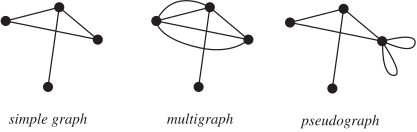
\includegraphics[scale=0.8]{images/graph-type-1}
        \caption{Phân biệt đơn đồ thị, đa đồ thị và giả đồ thị}
        \label{fig:graph-type-1}
    \end{center}
\end{figure}

\textit{Đồ thị vô hướng (undirected graph)} là đồ thị chứa các cạnh không định hướng. Nói cách khác, cạnh nối hai đỉnh x và y cũng sẽ được hiểu là cạnh đỉnh y với đỉnh x.

\textit{Đồ thị có hướng (directed graph)} là đồ thị chứa các cạnh có hướng. nói cách khác, cạnh nói hai đỉnh x và y sẽ phân biệt với cạnh nối từ y đến x.

\begin{figure}[H]
    \begin{center}
        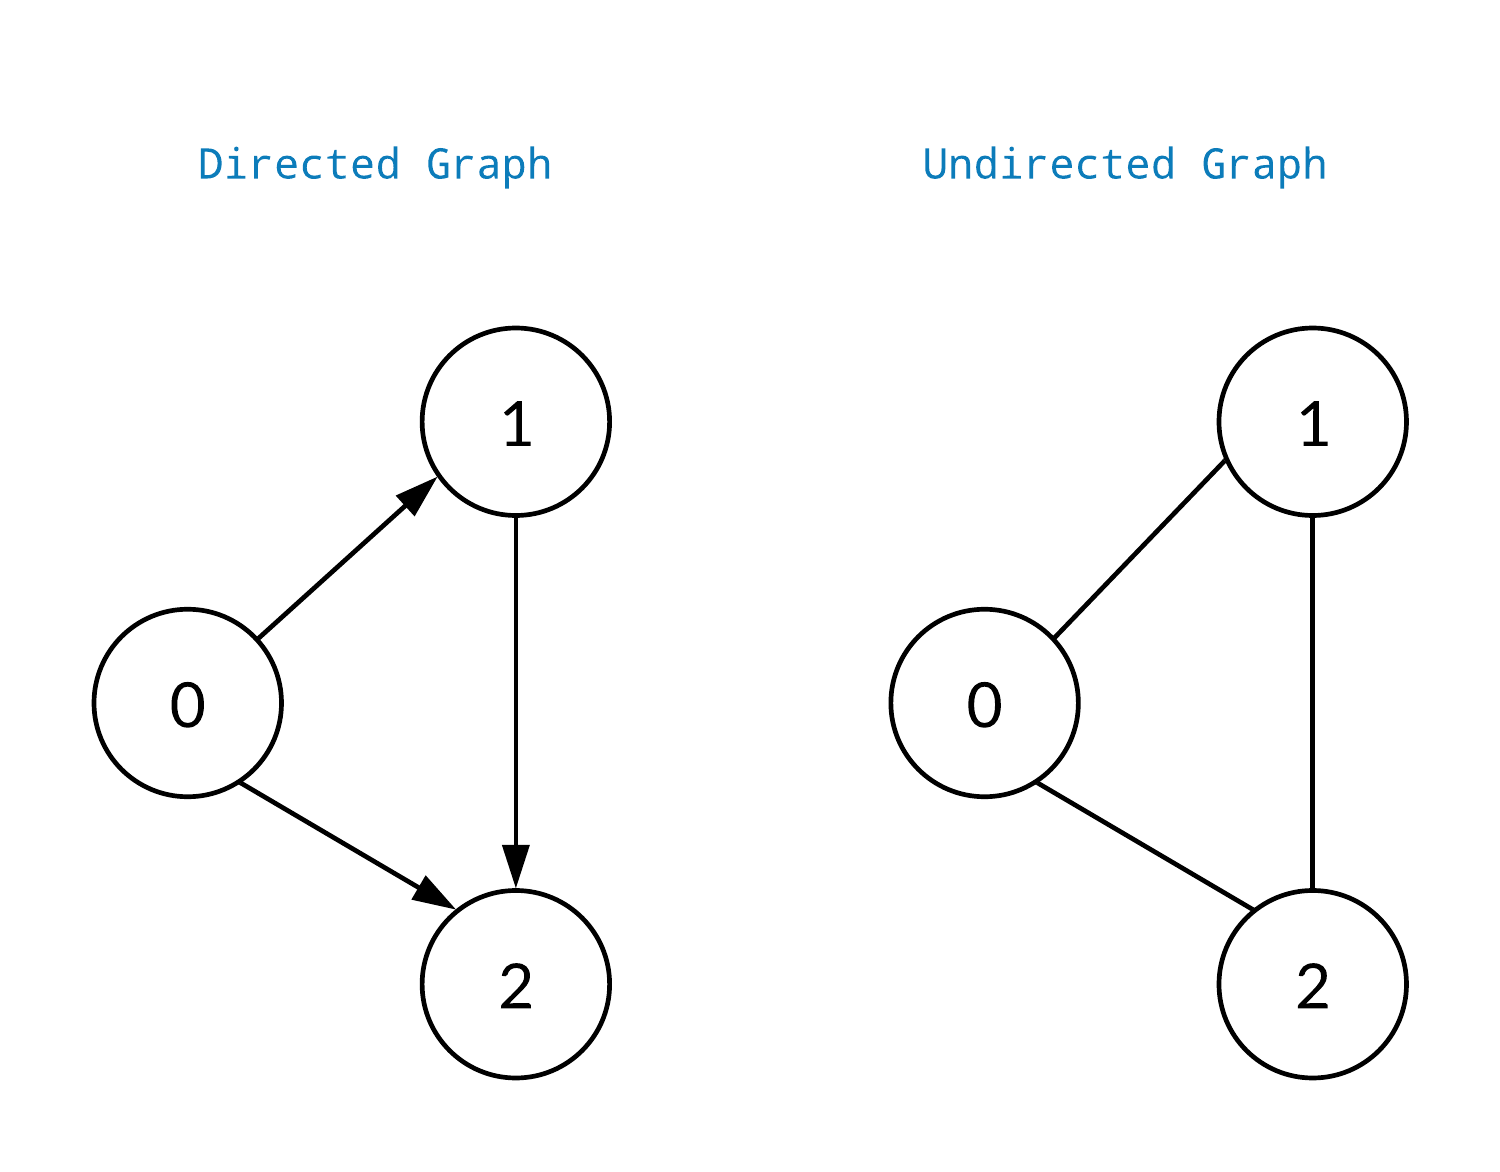
\includegraphics[scale=0.2]{images/graph-type-2}
        \caption{Phân biệt đồ thị vô hướng và đồ thị có hướng}
        \label{fig:graph-type-2}
    \end{center}
\end{figure}


Đồ thị có trọng số là đồ thị mà các cạnh của đồ thị được biểu diễn bằng một trọng số nào đó. Lúc này mỗi cạnh $e \in E$ sẽ được biểu diễn bởi $(x, y, w)$. Với x và y là hai đỉnh của cạnh và w là trọng số của cạnh đó

Đồ thị không trọng số là đồ thị mà các cạnh của đồ thị không được biểu diễn bởi một trọng số.

\begin{figure}[H]
    \begin{center}
        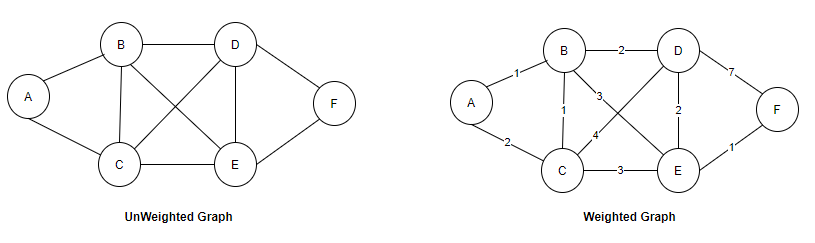
\includegraphics[scale=0.5]{images/graph-type-3}
        \caption{Phân biệt đồ thị có trọng số và không trọng số}
        \label{fig:graph-type-3}
    \end{center}
\end{figure}


Ngoài ra, khi kết hợp cách tính chất của các loại đồ thị khác nhau, ta có thể có được các dạng đồ thị khác như: Đơn đồ thị vô hướng, Đa đồ thị có hướng, Giả Đa đồ thị có hướng có trọng số,..

Đồ thị còn có thể phân loại theo đồ thị vô hạn và độ thị hữu hạn, chỉ số lượng cạnh và đỉnh của đồ thị là vô hạn hay có thể đếm được.

\subsubsection{Vector đặc trưng (feature vectors)}

Lý thuyết đồ thị khi được áp dụng vào các bài toán học máy thường sẽ được bổ sung thêm khác khái niệm vector đặc trưng. Vector đặc trưng là những vector chỉ các đặc trưng của một đỉnh hoặc một cạnh của đồ thị. Các vector đặc trưng biểu diễn cho các đối tượng giống nhau phải có số lượng chiều như nhau.

Các vector này có thể có một cấu trúc đã được định nghĩa trước với tập các trường được khảo sát trên đối tượng tương ứng với đỉnh đang xét. Ngoài ra các vector của có thể được huấn luyện nhờ vào các mô hình học máy. Một bài toán được quan tâm đến khi nhắc đến các vector đặc trưng này là từ các liên kết của đồ thị và các \textit{context vector} đã được định nghĩa trước, tìm ra các vector đặc trưng biểu diễn tốt cho các đối tượng đỉnh hoặc/và cạnh của đồ thị đó. Bài toán này được gọi là \textit{representation learning}.

\begin{figure}[H]
    \begin{center}
        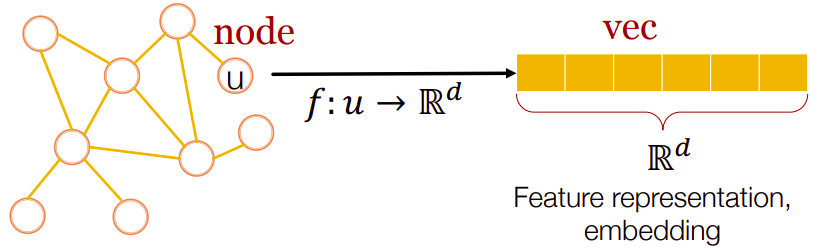
\includegraphics[scale=0.5]{images/feature-vector}
        \caption{Minh họa về vector đặc trưng}
        \label{fig:feature-vector}
    \end{center}
\end{figure}


\subsubsection{Ma trận kề (adjacent matrix)}

Ma trận kề là ma trận chứa các thông tin về các cạnh nối giữa các đỉnh trong đồ thị. Ma trận kề có kích thước $|V| \times |V|$. Phần tử ở hàng x cột y của ma trận chứa thông tin về kết nối giữa 2 đỉnh u và v và có giá trị như sau:
\begin{itemize}
	\item \textit{Đồ thị không trọng số}: 0 hoặc x biểu thị hoặc không có cạnh nối giữa 2 điểm u và v hoặc có x cạnh đang nối giữa 2 đỉnh này.
	\item \textit{Đồ thị có trọng số}: 0 hoặc w biểu thị hoặc không có cạnh nối giữa u và v hoặc có cạnh nối giữa u và v và trọng số của cạnh này là w.
\end{itemize}

\begin{figure}[H]
    \begin{center}
        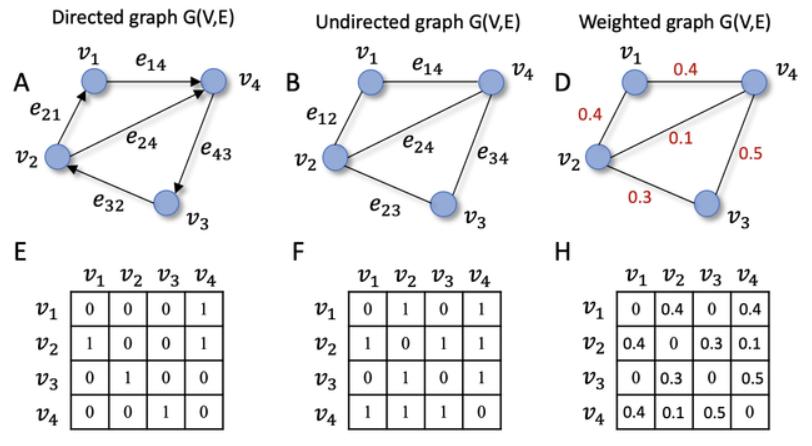
\includegraphics[scale=0.6]{images/adj-matrix}
        \caption{Ma trận kề}
        \label{fig:adj-matrix}
    \end{center}
\end{figure}


\subsubsection{Bậc của đồ thị}

Bậc của một đỉnh được định nghĩa là tổng số cạnh nối với đỉnh đó. Đối với đơn đồ thị, số cạnh nối với đỉnh đang xét cũng bằng số đỉnh kề với đỉnh đang xét. Bậc của đỉnh u được ký hiệu là $deg(u)$.

Tính chất:
\begin{itemize}
	\item Tổng số bậc của tất cả các đỉnh là số chẳn và có giá trị là $2m$ với m là số lượng cạnh của đồ thị:
	\begin{equation*}
		\sum_{v \in V}{deg(v)} = 2m
	\end{equation*}
	\item Tổng số đỉnh có bậc lẻ là số chẵn.
	\item Đối với đồ thị vô hướng, tổng giá trị của hàng x hoặc cột x của ma trận kề biểu diễn đồ thị đó chính bằng $deg(x)$
\end{itemize}

Đối với đồ thị có hướng, bậc của một đỉnh còn được phân ra làm 2 thành phần:
\begin{itemize}
	\item Bán bậc vào là số lượng cạnh nối với đỉnh đang xét và có hường vào đỉnh đó. Ký hiệu bán bậc vào của đỉnh u là $deg^-(u)$
	\item Bán bậc ra là số lượng cạnh nối với đỉnh đang xét và có hường ra khỏi đỉnh đó. Ký hiệu bán bậc ra của đỉnh u là $deg^+(u)$
\end{itemize}

\begin{equation*}
	deg(u) = deg^-(u) + deg^+(u)
\end{equation*}

\subsection{Mô hình Graph Convolution Network và bài toán representation learning}

Để giải bài toán \textit{representation learning} trên đồ thị, người ta đưa ra giả thuyết rằng, các nút trên đồ thị có khoảng cách càng gần nhau thì sẽ có các đặc tính giống nhau. Từ đó mà vector đặc trưng của những nút gần kế nhau cũng sẽ có khoảng cách gần nhau trong không gian latent.

\begin{figure}[H]
    \begin{center}
        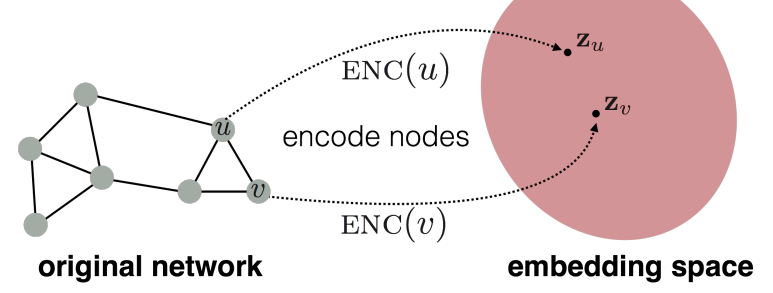
\includegraphics[scale=0.5]{images/representation-learning}
        \caption{Minh họa về bài toán \textit{Representation learning}}
        \label{fig:representation-learning}
    \end{center}
\end{figure}


Từ giả thuyết này, người ta đưa ra được ý tưởng chính của mạng \textit{GCN} là sử dụng các vector đặc trưng của các nút kề với nút đang xét để học được đặc trưng của nút này.

Cho đồ thị $G = (V,E)$, có ma trận kề $A_{n \times n}$ và ma trận đặc trưng $X_{n \times d}$ với $n = |V|$ và d là chiều của ma trận đặc trưng. Mô hình \textit{GCN} được kiến trúc bởi nhiều lớp ẩn chồng lên nhau. Gọi $H^{(l)}$ là đầu ra của lớp ẩn thứ l. $H^{(l)}$ là một ma trận có kích thức $n \times d_l$ với $d_l$ là số lượng đặc trưng của từng nút tại lớp $l$. Công thức tính $H^{(l)}$ được biểu diễn một như sau:
\begin{equation*}
	H^{(l)} = 
	\begin{cases}
		f(H^{(l-1)}, A), & l > 0 \\
		X, & l = 0		
	\end{cases}
\end{equation*}

Trong đó, $f$ là hàm tính đặc trưng của các nút dựa trên các lớp kề với nút đó. Do đó, $f$ có biểu diễn như sau:
\begin{equation*}
	f(H^{(l)}, A) = \sigma(AH^{(l)}W^{(l)})
\end{equation*}

Với $W$ là ma trận chứa các tham số học có kích thước $d_l \times d_{l+1}$. Và $\sigma$ là hàm kích hoạt phi tuyến của mô hình. 

Với công thức của hàm f như trên, ta thấy được 2 phần thiếu sót như sau:
\begin{itemize}
	\item Vector đặc trưng của nút u chỉ được tính bởi đặc trưng của các nút kề nó mà chưa được xét bởi các đặc trưng nội tại của nút u. Ta có thể giải quyết vấn đề này bằng các thêm các \textit{liên kết vòng (self loop)} từ một nút đến chính nó. Ta định nghĩa ma trận $\tilde{A}$ là ma trận kề của $G$ đã bổ sung các liên kết vòng:
	\begin{equation*}
		\tilde{A} = A + I
	\end{equation*} 
	\item Các đỉnh có bậc cao sẽ gây ảnh hưởng đến nhiều nút hơn các đỉnh khác. Và nó cũng sẽ được ảnh hưởng bởi nhiều đỉnh hơn các đỉnh khác. Theo như công thức $f$ ở trên, các đỉnh có bậc cao sẽ ma giá trị rất lớn hoặc rất nhỏ dẫn đến việc cập nhập gradient chậm lại trong quá trình lan truyền ngược. Để giải quyết vấn đề trên, \textit{GCN} sử dụng phép chuẩn hóa \textit{Symetric normalized Laplacian} để tránh sự thiên vị trong quá trình học.
	Từ đó mà ta có công thức đầy đủ của hàm f như sau:
	\begin{equation*}
		H^{(l+1)} = \sigma(\tilde{D}^{-1/2}\tilde{A}\tilde{D}^{1/2}H^{(l)}W^{(l)})
	\end{equation*}
\end{itemize}

Trong đó, $\tilde{D}$ là ma trận bậc của đồ thị $G$ phép chuẩn hóa đối xứng laplacian có thể được hiểu là với mỗi $\tilde{A}_{u,v}$ sẽ được nhân với một lượng $\frac{1}{\sqrt{deg(u)}\sqrt{deg(v)}}$


\subsection{Mô hình WordGCN}

\textit{WordGCN} là mô hình được ghép bởi 2 mô hình con là \textit{SynGCN} và \textit{SemGCN}. Cả hai mô hình trên đều áp dụng kiến trúc \textit{GCN} để trích xuất các \textit{embeddings} của các từ trong kho ngữ liệu. Trong khi \textit{SynGCN} trích xuất thông tin cú pháp (\textit{syntactic context}) của các từ thông qua các liên kết của chúng trong các đoạn văn bản. Thì \textit{SemGCN} rút trích các đặc trưng về ngữ nghĩa (\textit{semantic context}) của các từ thông qua các mối quan hệ như: đồng nghĩa, trái nghĩa, từ viết tắt,...

\subsubsection{Mô hình \textit{SynGCN}}

\textit{SynGCN} quan tâm đến đặc trưng của một từ thông qua ví trị và vai trò của từ đó trong câu. Theo \textit{Universal Dependency} \cite{2020arXiv200410643N} Mỗi từ trong câu sẽ có một,mmối quan hệ với một từ khác trong câu hoặc là chủ thể của cả câu (không có liên kết đến từ khác). Các mối quan hệ đó được gọi là các \textit{Universal Dependencies}. Từ đây, ta có thể xem mỗi câu $s = \{w_1, w_2,...,w_n\}$ trong kho ngữ liệu là một đồ thị con dạng cây có hướng $G_s = (V_s, E_s)$ với các nút là các từ $V_s=\{w_1, w_2, w_3...,w_n\}$ và các \textit{dependency} là các cạnh của đồ thị có dạng $(w_i, w_j, d_{ij})$ với $d_{ij}$ là mối quan hệ giữa $w_i$ và $w_j$. Lúc này, ta có thể áp dụng Thuật toán \textit{GCN} lên đồ thị này. 

\begin{figure}[H]
    \begin{center}
        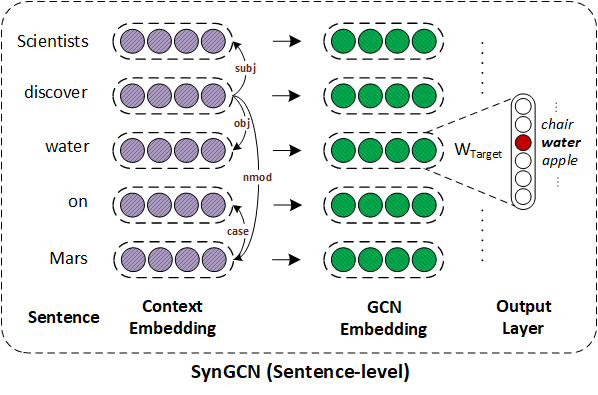
\includegraphics[scale=1.0]{images/syngcn_model}
        \caption{Mô hình cơ bản của \textit{SynGCN} \cite{wordgcn2019}}
        \label{fig:syngcn}
    \end{center}
\end{figure}


Nhận xét thấy \textit{GCN} áp dụng vào trường hợp này khá tương tự với mô hình \textit{Continues Bag of Word(CBOW)}. Mô hình này sử dụng tập các từ xung quanh $w_i$ để học các đặc trưng của $w_i$. Tập các từ như vậy được gọi là tập \textit{Context} của $w_i$.

\begin{equation*}
	C_{w_i} = \{w_{i+j}: -c \leq j \leq c, j \neq 0\}
\end{equation*}

Trong đó, $c$ là kích thước của cửa sổ trượt.

Đối với \textit{SynGCN}, tập \textit{Context} của $w_i$ được định nghĩa là tập các các từ tương ứng với nút kề với $w_i$:
\begin{equation*}
	C_{w_i} = N(w_i) = \{w_j: (w_i, w_j, l_{i,j}) \in E_s\}
\end{equation*}


\subsubsection{Mô hình SemGCN}

Các \textit{embedding} sau khi được huấn luyện qua mạng SynGCN sẽ được đưa vào mạng \textit{SemGCN} để học các đặc trưng về ngữ nghĩa (\textit{semantic context}). Mô hình cho phép học các mối quan hệ có tính đối xứng lẫn các mối quan hệ không đối xứng. Đối với các mô hình trước đây, hoặc là chúng chỉ có thể giải quyết các mối quan hệ đối xứng hoặc chưa xử lý tốt vối các môi không đối xứng. Gọi $G =(V,E)$ là đồ thị được tạo thành từ các ngữ nghĩa trong bộ dữ liệu. Ta sẽ có các đỉnh là các từ trong bộ nghữ liệu còn các cạnh là các mối quan hệ giữa chúng. Các cạnh trong G có định hướng. Đối với 2 từ x và y có liên kết đối xứng thì giữa 2 đỉnh tương ứng với x và y sẽ có 2 cạnh ngược hướng.

\begin{figure}[H]
    \begin{center}
        \includegraphics[scale=1.0]{images/SemGCN_model}
        \caption{Ý tưởng cơ bản của \textit{SemGCN} \cite{wordgcn2019}}
        \label{fig:SemGCN}
    \end{center}
\end{figure}


Sau khi có được đồ thì biểu diễn, ta có thể sử dụng thuật toán \textit{GCN} để tối ưu các \textit{embeddings} đã được huấn luyện từ mô hình \textit{SynGCN}.

\chapter{Phương pháp đề xuất}

\section{Áp dụng mô hình WordGCN vào mô hình Transformer}

Ở mô hình đề xuất, sinh viên muốn thay thể module mã hóa \textit{embedding} đầu vào và cả mã hóa \textit{embedding} đầu ra bằng các \textit{embedding} được huấn luyện thuông qua mô hình \textit{WordGCN}.

Ở mô hình đề xuất \textit{Transformer} \cite{transformer}, lớp mã hóa embedding đầu vào và đầu ra được cài đặt bằng một lớp feed forward. Ban đầu, các token được mã hóa bằng phương pháp \textit{onehot encoding}. Sau đó, được mã hóa thành các embedding của kích thước d = 512. 
Gọi $W$ có kích thước $n_{voc} \times d$ là ma trận trọng số của lớp mã hóa embedding đầu vào và đầu ra. Với $n_{voc}$ là số lượng từ vựng trong kho ngữ liệu và $d$ là số chiều của embedding. Embedding tương ứng với từ thứ i trong kho ngữ liệu được tính bằng công thức:
\begin{equation*}
	e_x = i_x \times W
\end{equation*}

Trong đó, $e_x$ là \textit{embedding} của từ thứ x còn $i_x$ là \textit{vector one-hot encoding} của từ thứ x.

\begin{figure}[H]
    \begin{center}
        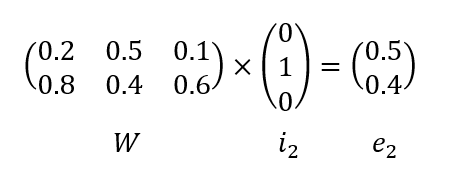
\includegraphics[scale=0.8]{images/original_input_embedding}
        \caption{Minh họa lớp mã hóa embedding với số lượng từ vựng trong kho ngữ liệu $n_{voc} = 3$ và số chiều của embedding $d = 2$}
        \label{fig:original-input-embedding}
    \end{center}
\end{figure}

Các tiếp cận này chưa khai thác được các đặc trưng về cú pháp và các đặc trưng về ngữ nghĩa của các từ vựng trong một ngôn ngữ. Bằng cách sử dụng WordGCN, các embeddings sẽ được huấn luyện trước qua 2 mô hình \textit{SynGCN} và \textit{SemGCN}. Kết quả sẽ được lưu vào trong một tập tin. Sau đó được truyền truyền thẳng vào mô hình  \textit{transformer} .

(Hình minh họa quá trình)

\section{Chuẩn bị dữ liệu}

\subsection{Tập dữ liệu WMT14}
\textit{WMT14 (Workshop on Statistical Machine Translation 2014)} \cite{wmt14} là một workshop chia sẻ về các bài toán được quan tâm trong lĩnh vự dịch máy. Trong đó, có 4 bài toán:
\begin{itemize}
	\item Translation task 
	\item Quality estimation task 
	\item metric task 
	\item Medical translation task
\end{itemize}

Trong phạm vi của khóa luận, sinh viên quan tâm đến bài toán dịch máy (translation task) với 2 ngôn ngữ là tiếng Anh và tiếng Đức. 

Với tập dữ liệu huấn luyện, WMT14 đã cung cấp khoảng 4.5 triệu câu từ 3 kho ngữ liệu song ngữ Anh-Đức:
\begin{itemize}
	\item Kho ngữ liệu song ngữ \textit{Europarl}: Được trích xuất từ các thủ tục hành chính của nghị viện Châu Âu
	\item Kho ngữ liệu song ngữ \textit{News Commentary}: bao gồm bình luận chính trị và kinh tế được thu thập từ trang web Project Syndicate
	\item Kho ngữ liệu song ngữ \textit{Common Crawl}: bao gồm các thông tin được thu thập từ tổng hợp các nguồn trên internet.
\end{itemize}

Với tập dữ liệu kiểm thử, dữ liệu được tổng hợp từ các mẫu truyện từ internet. Theo \cite{wmt14}, tập kiểm thử bao gồm 1500 câu tiếng Anh được dịch sang tiếng Đức và 1500 câu tiếng Đức được dịch về tiếng anh. Các mẫu dịch được cung cấp bởi các chuyên gia từ \textit{Capita}. 

\begin{table}[H]
	\centering
    \caption{Bảng thống kê số liệu của kho ngữ liệu song ngữ \textit{Europarl}}
    \label{tab:Europarl}
	\begin{tabular}{l|cc|}
	\cline{2-3}
		& \multicolumn{2}{c|}{\textbf{German $\leftrightarrow$ English}} \\ \hline
		\multicolumn{1}{|l|}{\textbf{Sentences}} & \multicolumn{2}{c|}{1,920,209} \\ \hline
		\multicolumn{1}{|l|}{\textbf{Words}}          & \multicolumn{1}{c|}{50,486,398} & 53,008,851 \\ \hline
		\multicolumn{1}{|l|}{\textbf{Distinct words}} & \multicolumn{1}{c|}{381,583} & 115,966 \\ \hline
	\end{tabular}
\end{table}

\begin{table}[H]
	\centering
	\centering
    \caption{Bảng thống kê số liệu của kho ngữ liệu song ngữ \textit{New Commentary}}
   \caption{}
    \label{tab:New Commentary}
	\begin{tabular}{l|cc|}
		\cline{2-3}
		& \multicolumn{2}{c|}{\textbf{German $\leftrightarrow$ English}} \\ \hline
		\multicolumn{1}{|l|}{\textbf{Sentences}}      & \multicolumn{2}{c|}{201,288}                  \\ \hline
		\multicolumn{1}{|l|}{\textbf{Words}}          & \multicolumn{1}{c|}{5,105,101}   & 5,046,157  \\ \hline
		\multicolumn{1}{|l|}{\textbf{Distinct words}} & \multicolumn{1}{c|}{150,760}     & 65,520     \\ \hline
	\end{tabular}
\end{table}

\begin{table}[H]
	\centering
    \caption{Bảng thống kê số liệu của kho ngữ liệu song ngữ \textit{Common Crawl}}
    \label{tab:Common Crawl}
	\begin{tabular}{l|cc|}
	\cline{2-3}
	& \multicolumn{2}{c|}{\textbf{German $\leftrightarrow$ English}} \\ \hline
	\multicolumn{1}{|l|}{\textbf{Sentences}}      & \multicolumn{2}{c|}{2,399,123}               \\ \hline
	\multicolumn{1}{|l|}{\textbf{Words}}          & \multicolumn{1}{c|}{54,575,405} & 58,870,638 \\ \hline
	\multicolumn{1}{|l|}{\textbf{Distinct words}} & \multicolumn{1}{c|}{1,640,835}  & 823,480    \\ \hline
	\end{tabular}
\end{table}

\subsection{Tiền xử lý dữ liệu cho mô hình SynGCN}

\subsubsection{Định dạng của dữ liệu}

Theo \cite{github.wordgcn}, dữ liệu đầu vào của \textit{SynGCN} phải được tiền xử lý thành các tập tin có cấu trúc như sau:
\begin{itemize}
	\item \textit{voc2id.txt}: Gán id cho mỗi từ trong kho từ vựng
	\begin{equation*}
		voc2id: W \rightarrow \mathbb{R}
	\end{equation*}
	\item \textit{id2freq.txt}: Thống kê tần số xuất hiện của các từ vựng không kho ngữ liệu
	\item \textit{de2id.txt}: Gán id cho các mối quan hệ trong universal dependencies
	\item \textit{data.txt}: Biểu diễn lại kho ngữ liệu theo định dạng:
	\begin{equation*}
	N\ M\ tok_1\ tok_2\ tok_3 ... tok_N\ dep_1\ dep_2 .... dep_M
	\end{equation*}
	\begin{itemize}
		\item N là số lượng từ trong câu và M là số lượng mối quan hệ giữa các từ trong câu.
		\item $tok_i$ là id của từ thứ i trong câu.
		\item $dep_i$ là mối quan hệ thứ i trong câu. Mỗi mối quan hệ được biểu diễn dưới dạng:
		\begin{equation*}
			source\_token|destination\_token|dep\_rel\_label
		\end{equation*}
		Trong đó, \textit{source\_token} và \textit{destination\_token} là hai từ phát sinh mối quan hệ với nhau. \textit{dep\_rel\_label} là mối quan hệ giữa hai từ này.
	\end{itemize}
\end{itemize}

\subsubsection{Voc2id}

WMT14 đã cung cấp sẵn cho ta tập V là tập hợp các từ vựng trong kho ngữ liệu. Do đó, ta chỉ cần đánh số thứ tự cho các từ trong V.

\begin{algorithm}[H]
    \caption{Tiền xử lý dữ liệu voc2id}
    \begin{algorithmic}[1]
		\State Khởi tạo $tok_{<unk>} = 0$
		\State Khởi tạo $count \gets 1$
		\For{$w \in V$}
			\State $tok_{w} = count$
			\State $count \gets count + 1$
		\EndFor
    \end{algorithmic}
\end{algorithm}

\subsubsection{id2freq}

\begin{algorithm}[H]
    \caption{Tiền xử lý dữ liệu id2freq}
    \begin{algorithmic}[1]
		\State Khởi tạo $\forall w \in V : freq_w = 0$
		\State Khởi tạo $freq_{<unk>} = 0$
		\For{$w \in W$}
			\If{$w \in V$} 
				\State $freq_{w} \gets freq_{w} + 1$
			\Else 
				\State $freq_{<unk>} \gets freq_{<unk>} + 1$
			\EndIf
		\EndFor
    \end{algorithmic}
\end{algorithm}

Trong đó, \textit{<unk>} là các từ lạ không nhận diện được từ bộ từ vựng.

\subsubsection{de2id}

Tập các mối quan hệ $Dep$ được tổng hợp từ \textit{Universal dependencies}.

\begin{algorithm}[H]
    \caption{Tiền xử lý dữ liệu de2id}
    \begin{algorithmic}[1]
		\For{$relation \in Dep$}
			\State $dep_{relation} = count$
			\State $count \gets count + 1$
		\EndFor
    \end{algorithmic}
\end{algorithm}

\subsubsection{data}

Theo \textit{WordGCN}, để có thể rút trích các mối quan hệ của các từ trong câu, ta sử dụng công cụ \textit{CoreNLP Parser}. Ở bước này, do các câu có thể xử lý một các độc lập nhau. Ta có thể chia tập dữ liệu ra thành các tập nhỏ hơn để xử lý giúp tăng hiệu quả tính toán và giảm gánh nặng tài nguyên. Các phần cứng chạy song song sẽ chia sẻ với nhau chung các tập tin \textit{voc2id}, và \textit{de2id}. Mỗi máy thành phần thứ $i$ sẽ được xử lý tập $S_i \subset S$ với $S$ là tập tất cả các câu trong kho ngữ liệu.


\begin{algorithm}[H]
    \caption{Tiền xử lý dữ liệu data}
    \begin{algorithmic}[1]
		\State $document = CoreNLP\_Parser(S_i)$
		\For{$sentence \in document$}
			\State Ghi số lượng từ trong câu vào data.txt
			\State Ghi số lượng quan hệ trong câu vào data.tx
			\For{$word \in sentence$}
				\If{$word \in V$}
					\State Ghi $tok_{word}$ vào data.txt
				\Else
					\State Ghi $tok_{<unk>}$ vào data.txt
				\EndIf
			\EndFor

			\For{$dep \in dependencies(sentence)$}
				\State Ghi $dep_{src}|dep_{dest}|dep_{relation}$ vào data.txt
			\EndFor
			
			\State Writeln
		\EndFor
    \end{algorithmic}
\end{algorithm}

\subsection{Tiền xử lý dữ liệu cho mô hình SemGCN}

\subsubsection{WordNet}

WordNet là kho ngữ liệu từ vựng gom nhóm các từ tương đồng thành các tập gọi là các synsets. Các từ trong một synset có thể được thay đổi cho nhau mà không làm thay đổi ý nghĩa của câu ở một số trường hợp nhất định.

Các mối quan hệ được đề cập trong WordNet chủ yếu là thượng-hạ vị. Ngoài ra còn cung cấp thêm các cặp từ trái nghĩa.

Khái niệm hạ vị chỉ một từ hoặc một cụm từ có ngữ nghĩa được kế thừa từ một từ khác. Từ đó, ta có khái niệm thượng vị là một từ có ngữ nghĩa chứa đựng ngữ nghĩa của một từ khác. Có thể thấy, thượng \- hạ vị là các mối quan hệ không đối xứng, và không thể có một từ vừa là thượng vị cũng vừa là hạ vị của một từ. Từ đó, ta có thể tạo ra được một rừng (tập hợp của các đồ thị con dạng cây) có hướng. Với các đỉnh cha là thượng vị của các đỉnh con.

Ngoài ra, ta còn có khái niệm đồng hạ vị (co-hyponym) chỉ các cặp từ cùng là hạ vị của một từ.

\begin{figure}[H]
    \begin{center}
        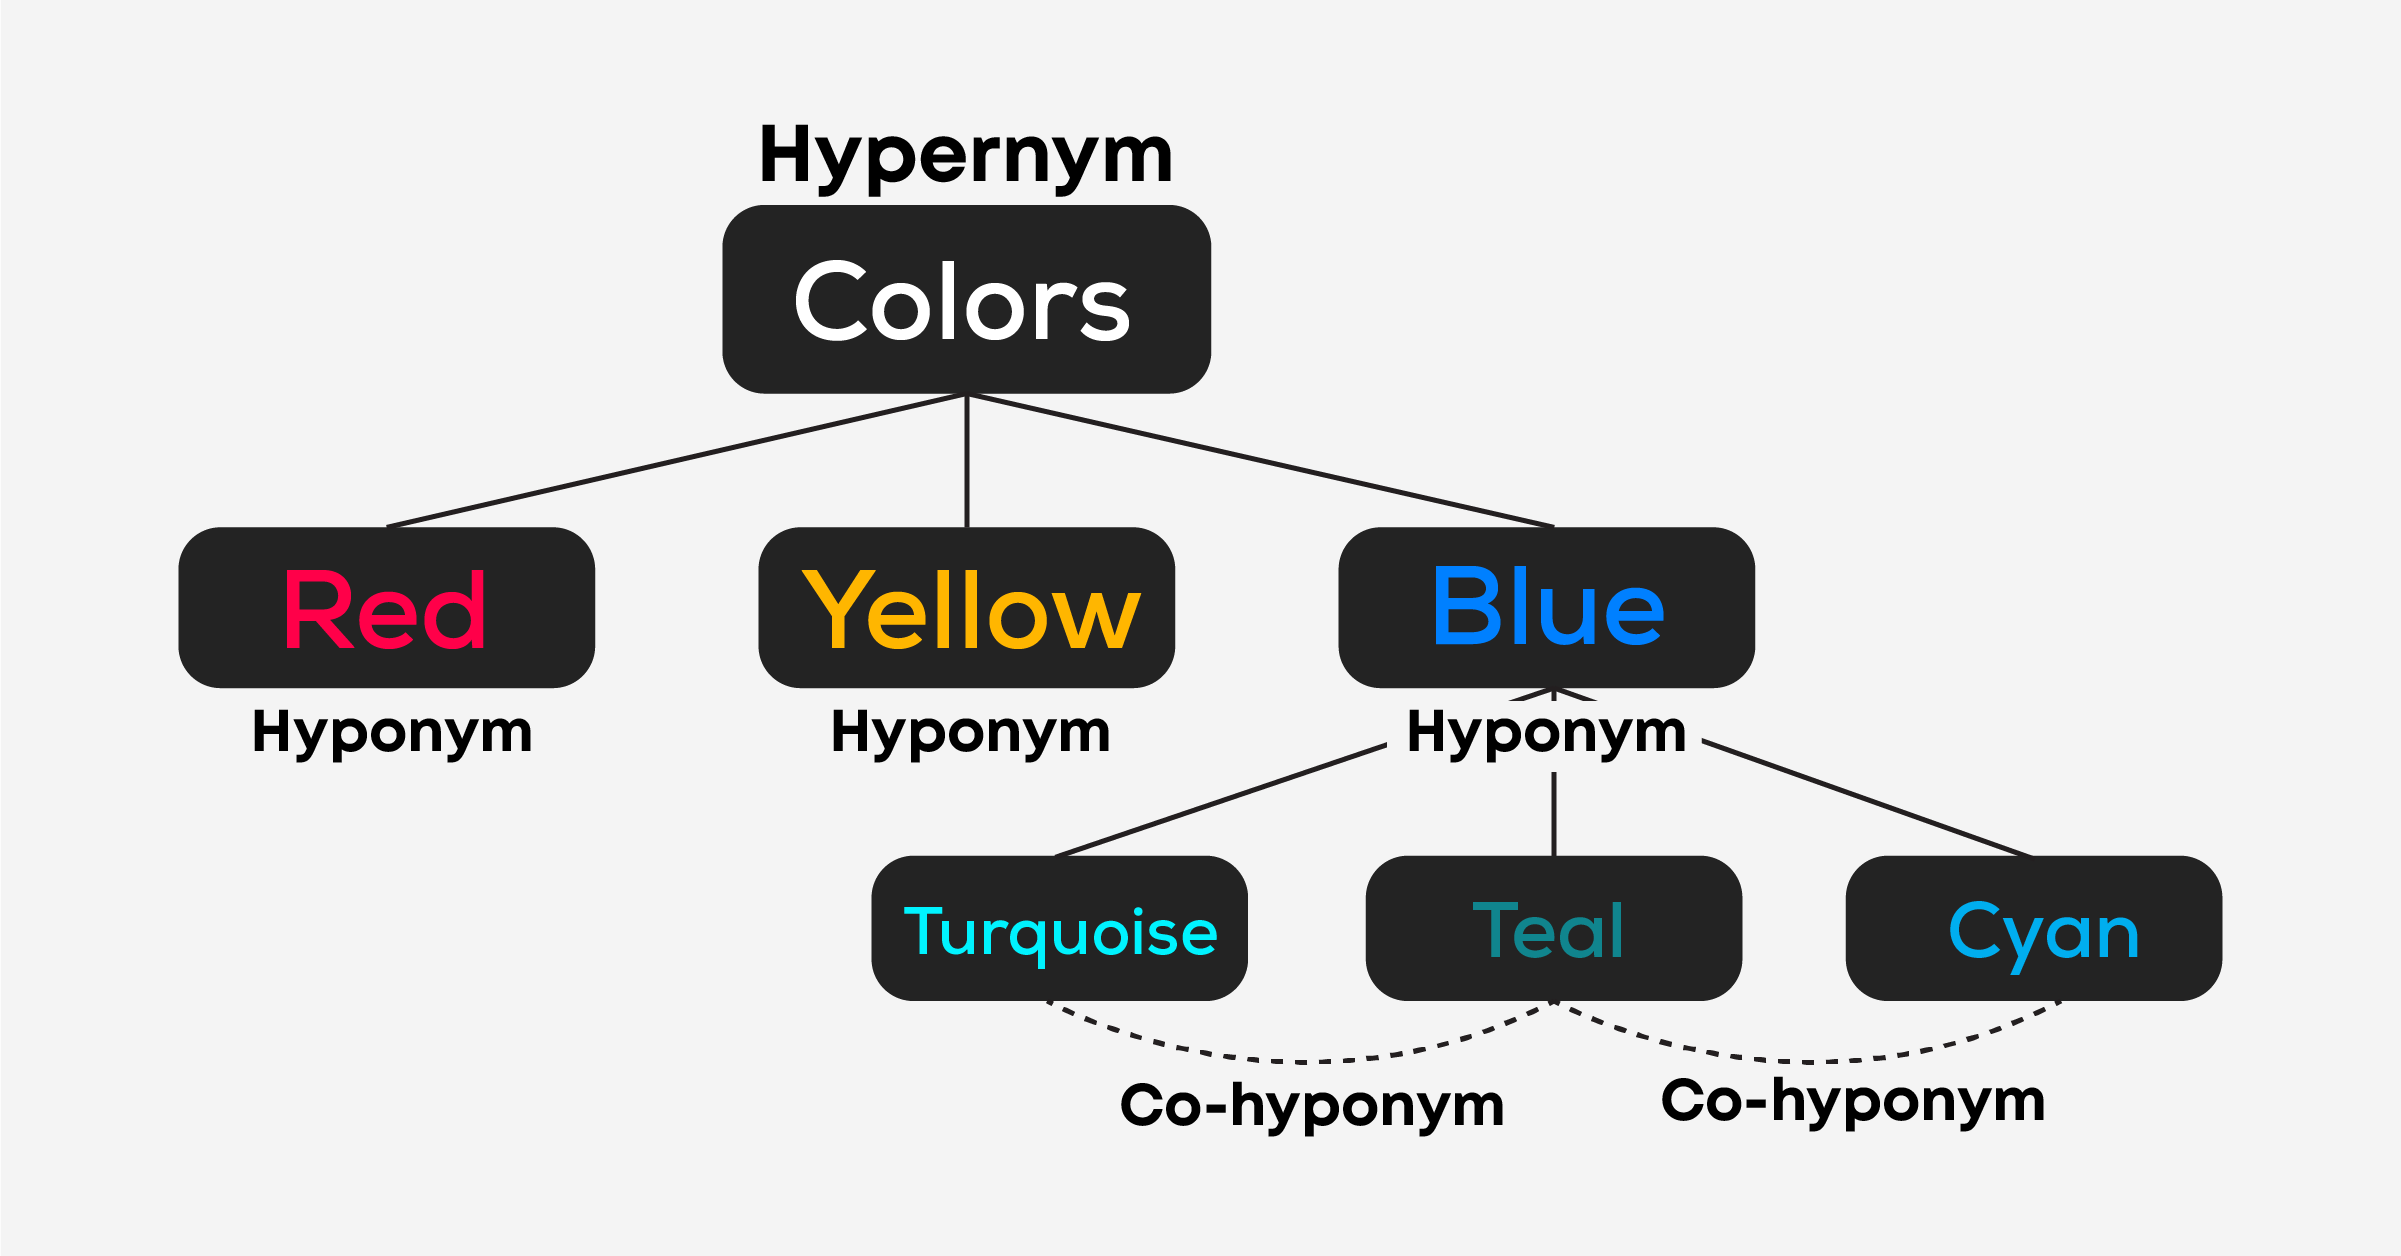
\includegraphics[scale=0.185]{images/hypernym-hyponym}
        \caption{Ảnh minh họa thượng vị và hạ vị}
        \label{fig:hypernym-hyponym}
    \end{center}
\end{figure}

Theo như ví dụ trên, các màu sắc "red" (đỏ), "yellow" (vàng) và "blue" (xanh dương) là các hạ vị của "colors" (màu sắc) do chúng đều có ý nghĩa là một màu sắc. "Colors" được gọi là thượng vị của "red", "yellow" và "blue". Bên cạnh đó, "yellow" và "blue" do có chung một thượng vị nên chúng được gọi là đồng thượng vị.


\subsubsection{Định dạng dữ liệu}

Theo \cite{github.wordgcn}, \textit{SemGCN} quan tâm đến 4 mối quan hệ ngữ nghĩa và được xác định bởi 4 tập tin sau:
\begin{itemize}
	\item \textit{Antonyms}: bao gồm các cặp từ có ý nghĩa trái ngược nhau trong kho từ vựng. Mối quan hệ trái nghĩa là mối quan hệ 2 chiều và sẽ biểu diễn bằng 2 cạnh đối nhau trong đồ thị ngữ nghĩa.
	\item \textit{Hypernyms}: chứa các cặp bao gồm một từ và thượng vị của nó. Mối quan hệ này là mối quan hệ một chiều.
	\item \textit{Hyponyms}: chứa các cặp từ bao gồm một từ và một hạ vị của nó. Mối quan hệ này cũng là moios quan hệ một chiều.
	\item \textit{Synonyms}: bao gồm nhiều dòng, với mỗi dòng biểu diễn một từ và tập các từ đồng nghĩa với từ đó.
\end{itemize}

Dựa trên \textit{WordGCN}, các mối quan hệ \textit{antonyms, hypernym} và \textit{hyponym} được trích xuất nhờ vào WordNet, còn mối quan hệ \textit{synonym} thì được trích xuất dựa vào PPDB (The paraphrase database).

\subsection{Tiền xử lý dữ liệu cho mô hình transformer}

Dữ liệu đầu vào của \textit{transformer} bao gồm 2 phần:
\begin{itemize}
	\item kho ngữ liệu WMT14 bao gồm các cặp câu song ngữ Anh-Đức.
	\item Các embedding được huấn luyện bởi mô hình WordGCN
\end{itemize}

Với dữ liệu WMT14, ta cần thực hiện tokenization các từ trong kho ngữ liệu với id của các từ phải tương ứng với id trong tập tin voc2id.txt. Ngoài ra, ta phải bổ sung thêm ba token đặc biệt vào vào bộ từ vựng như sau:
\begin{itemize}
	\item \textit{<pad>}: Ma trận chứa dữ liệu đầu vào của  \textit{transformer}  có kích thước $n \times len\_max$. Trong đó n là số lượng câu còn $len\_max$ là kích thước của câu có chiều dài dài nhất trong kho ngữ liệu. Do đó, dẫn đến một số hàng của ma trận sẽ không có giá trị. Ta bổ sung thêm một token đặc biệt này vào để lắp đầy các vị trí đó. Embedding tương ứng với \textit{<pad>} sẽ được gán giá trị bằng với vector 0.
	\item \textit{<bos>}: Token này dùng để đánh dấu bắt đầu của một câu. Giá trị của Embedding tương ứng sẽ được gán là vector với toàn giá trị 1 ở mọi chiều.
	\item \textit{<eos>}: token này dùng để đánh dấu kết thúc của một câu. Giá trị của Embedding tương ứng sẽ được gán là vector với toàn giá trị -1 ở mọi chiều.
\end{itemize}

\begin{figure}[H]
    \begin{center}
        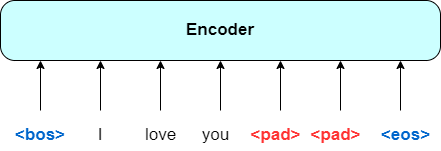
\includegraphics[scale=0.85]{images/special-token}
        \caption{Minh họa về các token đặc biệt trong mô hình \textit{transformer} }
        \label{fig:special token}
    \end{center}
\end{figure}

Dữ liệu các embedding đã được huấn luyện bởi mô hình WordGCN sẽ được lưu trữ trong một tập tin có dạng như sau:

\begin{figure}[H]
    \begin{center}
        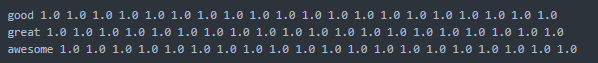
\includegraphics[scale=1]{images/pretrained-embedding}
        \caption{Định dạng của tập tin chứa các \textit{embedding} được huấn luyện bởi mô hình \textit{WordGCN}. Ở ví dụ này mỗi từ được biểu diễn bởi một embedding của số chiều là 20.}
        \label{fig:pretrained-embedding}
    \end{center}
\end{figure}

Mỗi dòng sẽ chứa thông tin về \textit{embedding} của một từ trong kho ngữ liệu. Trong đó:
\begin{itemize}
	\item Một từ đầu dòng thuộc kho ngữ liệu.
	\item $d$ số tiếp theo biểu thị giá trị của \textit{vector embedding} của từ đang xét.
\end{itemize}

\chapter{Huấn luyện và Kết quả}

\section{Huấn luyện}

Như đã trên bày ở trên, cả 2 mô hình \textit{WordGCN} và  \textit{Transformer}  đều sẽ được huấn luyện bởi kho ngữ liệu \textit{WMT14}. Với khoảng 4.5 triệu câu song ngữ Anh Đức. Sử dụng bộ tự vựng bao gồm 50000 từ cho cả 2 ngôn ngữ Anh và Đức.

\subsection{Kích thước batch của dữ liệu huấn luyện}
Kích thước batch của dữ liệu được huấn luyện đối với mô hình \textit{SynGCN} là 128 và mô hình \textit{SemGCN} là 64. 

Đối với \textit{Transformer}, mỗi batch dữ liệu sẽ có kích thước 25000.

\subsubsection{Thuật toán tối ưu}
\textit{SynGCN} và \textit{SemGCN} sử dụng thuật toán \textit{Adam} với giá trị của \textit{learning rate}:
\begin{equation*}
	l_{rate} = 10^{-3}
\end{equation*}

Đối với \textit{Transformer}, thuật toán tối ưu được sử dụng vẫn là \textit{Adam} với các siêu tham số như sau:
\begin{equation*}
	\begin{cases}
		l_{rate} = 10^{-3} \\
		\beta_1 = 0.9 \\
		\beta_2 = 0.98 \\
		\epsilon = 10^{-9}
	\end{cases}
\end{equation*}

\subsection{Kết quả}

\begin{table}[H]
\centering
\begin{tabular}{ll}
	\multicolumn{1}{c|}{Mô hình}                 & \multicolumn{1}{c}{BLEU}  \\ \hline
	\multicolumn{1}{l|}{ \textit{transformer} (baseline)}           & \multicolumn{1}{l}{27.3} \\ \hline
	\multicolumn{1}{l|}{WordGCN +  \textit{transformer} } & \multicolumn{1}{l}{26.5} \\ \hline
\end{tabular}
\caption{Bảng kết quả huấn luyện của mô hình cơ sở và mô hình đề xuất}
\end{table}

Kết quả huấn luyện của mô hình đề xuất tuy chưa thể vượt qua được kết quả của mô hình cơ sở tuy nhiên vẫn có hiệu quả khá tốt so với các mô hình trước đây. Nguyên nhân của kết quả này có thể là do các nguyên nhân sau:
\begin{itemize}
	\item Các bộ siêu tham số chưa được tối ưu giá trị.
	\item Kho từ vựng còn thiếu sót nhiều từ.
	\item Kích thước embedding được huấn luyện ở mô hình \textit{WordGCN} chưa phù hợp khi đưa vào mô hình \textit{transformer} .
\end{itemize}

\chapter{Kết luận}

Qua khóa luận này, sinh viên đã nghiên cứu về các thuật toán học sâu trên các bộ dữ liệu non-Euclidean (Graph Neural Network). Cụ thể hơn là mô hình WordGCN, được cấu thành bởi 2 mô hình con là \textit{SynGCN} và \textit{SemGCN}. Cả 2 mô hình con đều được lấy ý tưởng từ một biến thể thường gặp của Graph Neural Network đó là Graph Convolutional Network.

Ngoài ra, sinh viên còn nghiên cứu về bài toán học máy. Hướng nghiên cứu là về mô hình  \textit{transformer} . Một mô hình dịch máy dựa hoàn toàn vào cơ chế attention, bỏ qua các kiến trúc kinh điển như mạng tích chập hay mạng hồi quy.

Cuối cùng, sinh viên đề xuất sử dụng các word embedding được huấn luyện từ mô hình WordGCN để áp dụng vào mô hình  \textit{transformer}  với mục đích sử dụng các thông tin về cú pháp và ngữ nghĩa từ các embedding này làm tăng hiệu năng của mô hình  \textit{transformer} .

\textbf{Định hướng phát triển}. Kết quả tuy chưa đạt được như kì vọng, song đã đống góp được ý tưởng để phát triển các thuật toán xử lý ngôn ngữ tự nhiên trong tương lai. Có thể thấy tiềm năng của việc sử dụng các word embedding được huấn luyện bởi các mô hình non-Euclidean có thể áp dụng cho không chỉ các thuật toán dịch máy mà còn cho các thuật toán khác. Một số bài toán đang được quan tâm như: 
\begin{itemize}
	\item Phân tích các bình luận 
	\item Các bài toán về gợi ý phim ảnh, bài hát, sản phẩm,\dots
	\item Bài toán tự động điền của các công cụ tìm kiếm như Google, Bing,\dots
	\item Bài toán phát hiện email rác, gợi ý trả lời email.
\end{itemize} 

% Công trình của tác giả (nếu không có thì comment 02 dòng dưới)
% \addcontentsline{toc}{chapter}{Danh mục công trình của tác giả}
% \chapter*{Danh mục công trình của tác giả}
\label{Appendix1}

\begin{enumerate}
\item Tạp chí ABC
\item Tạp chí XYZ
\end{enumerate}

% In tài liệu tham khảo
\addcontentsline{toc}{chapter}{Tài liệu tham khảo}
\printbibheading[title={Tài liệu tham khảo}]

\printbibliography[heading=subbibliography, title={Tiếng Việt}, keyword=Viet, resetnumbers=true]

\DeclareNameAlias{sortname}{last-first}
\DeclareNameAlias{default}{last-first}

\printbibliography[heading=subbibliography, title={Tiếng Anh}, notkeyword=Viet, resetnumbers=4] 
% ===================================================================== %
% CHÚ Ý: phải gán lại resetnumbers=số tài liệu tham khảo tiếng Việt + 1 %
% ===================================================================== %

% Phần phụ lục
%\appendix

\chapter{Ngữ pháp tiếng Việt}
\label{Appendix1}

Đây là phụ lục.
%\chapter{Ngữ pháp tiếng Nôm}
\label{Appendix2}

Đây là phụ lục 2.

\end{document} 